% Define document class
\documentclass[modern]{aastex631}

% Custom defs
% Packages
\usepackage{xifthen}
\usepackage{array}
\usepackage{upgreek}
\usepackage[bbgreekl]{mathbbol}
\usepackage{afterpage}
\usepackage[bb=boondox]{mathalpha}
\usepackage{tipa}
\usepackage{booktabs}


% Shorthand for this paper
\newcommand{\starry}{\textsf{starry}\xspace}
\newcommand{\Python}{\textsf{Python}\xspace}
\newcommand{\cpp}{\textsf{C}++\xspace}
\newcommand{\bvec}[1]{{\ensuremath{\mathbf{#1}}}}
\newcommand{\xxx}[1]{{\color{red}#1}}
\DeclarePairedDelimiter\floor{\lfloor}{\rfloor}
\DeclarePairedDelimiter\ceil{\lceil}{\rceil}
\newcommand{\imag}{{\ensuremath{\mathbb{i}}}}
\renewcommand{\quad}{\hskip 0.33em}
\newcommand{\quadquad}{\quad\quad\quad\quad}

\newcommand{\R}{\bvec{R}}
\newcommand{\AOne}{\bvec{A_1}}
\newcommand{\alm}{\bvec{a}}
\newcommand{\x}{\bvec{x}}
\newcommand{\D}{D}
\newcommand{\Doppler}{\bvec{D}}
\newcommand{\Surf}{\mathcal{S}}
\newcommand{\Curve}{\mathcal{C}}
\newcommand{\Dargs}{\bvec{d}}
\newcommand{\lmax}{\ensuremath{l_\mathrm{max}}}
\newcommand{\spot}{\texttt{SPOT}\xspace}
\newcommand{\vogtstar}{\texttt{VOGTSTAR}\xspace}
\newcommand{\kT}{\boldsymbol{\kappa}^\top}
\newcommand{\rhoT}{\boldsymbol{\rho}^\top}
\newcommand{\ylmbasis}{\boldsymbol{\psi}^\top}
\newcommand{\pbasis}{\boldsymbol{\phi}^\top}
\newcommand{\pbasisn}{\ensuremath{\phi_n}}
\newcommand{\almt}{\ensuremath{\bvec{a}}}
\newcommand{\lnlam}{\mbox{\textipa{\textcrlambda}}}

% TIMING RESULTS
\def\timeInferY{under 1 second}
\def\timeInferYB{about 5 seconds}
\def\timeInferYBS{about 30 seconds}
\def\timeInferYBSLOSNR{about 30 seconds}
\def\timeInferTwoSpec{about 20 minutes}

% Begin!
\begin{document}

% Title
\title{A Closed-Form Solution to the Doppler Imaging Problem}

% Author list
\author[0000-0002-0296-3826]{Rodrigo Luger}
\email{rluger@flatironinstitute.org}
\affil{Center~for~Computational~Astrophysics, Flatiron~Institute, New~York, NY}
%
\author[0000-0001-9907-7742]{Megan Bedell}
\affil{Center~for~Computational~Astrophysics, Flatiron~Institute, New~York, NY}
%
\author[0000-0002-9328-5652]{Daniel Foreman-Mackey}
\affil{Center~for~Computational~Astrophysics, Flatiron~Institute, New~York, NY}
%
\author[0000-0002-1835-1891]{Ian Crossfield}
\affil{Department~of~Physics~and~Astronomy, Kansas University, Lawrence, KS}
%
\author[0000-0002-3852-3590]{Lily Zhao}
\affil{Center~for~Computational~Astrophysics, Flatiron~Institute, New~York, NY}
%
\author[0000-0003-2866-9403]{David W. Hogg}
\affil{Center~for~Computational~Astrophysics, Flatiron~Institute, New~York, NY}

\begin{abstract}
    We derive a novel, efficient, and closed form solution to the problem of Doppler imaging of stellar surfaces from high resolution spectral timeseries datasets.
    %
    Our model for the observed spectrum is linear in the parameters describing the specific intensity distribution on the surface, which makes the posterior over surface maps computationally trivial to evaluate under certain choices of priors.
    %
    Our model is also linear in the local (rest frame) stellar spectrum, which may itself be spatially variable; this allows one to perform Doppler imaging with limited knowledge of the local stellar spectrum and therefore works on blended lines, regions of the spectrum where line formation mechanisms are not well understood, or stars whose spots have intrinsically different spectra from the rest of the photosphere.
    %
    We implement the model within the open-source \starry stellar modeling framework, making it fast, differentiable, and easy to use in both optimization and posterior inference settings.
    %
    As a proof-of-concept, we use our model to infer the surface map of the brown dwarf Luhman 16B, finding close agreement with the solution of \citet{Crossfield2014}.
    %
    %While our derivation neglects the effects of differential rotation and convective blueshift, these are straightforward to include and will be addressed in an upcoming paper, which will also extend the present formalism to the problem of Doppler tomography.
    %
    This paper was prepared using the \texttt{showyourwork} scientific article workflow, which exposes the data, source code, and package dependencies for all of the paper's figures, allowing readers to reproduce the results in this paper exactly and with minimal effort.
\end{abstract}

% Main body
\section{Introduction}

\xxx{%
    \noindent Introduce the problem of Doppler imaging.
    Then cite the following papers:\\[0.5em]
    \noindent\textbf{Misc.} \\
    \noindent\citet{Luger2019} --- Surface modeling with spherical harmonics: \starry \\
    \noindent\citet{Bedell2019} --- Data-driven spectral inference: \texttt{wobble} \\[0.5em]
    %
    \noindent\textbf{Theory} \\
    \noindent\citet{Khokhlova1976,Goncharskii1977} --- Local line profile from observed spectrum\\
    \noindent\citet{Vogt1983,Vogt1987} --- Seminal papers on Doppler imaging \\
    \noindent\citet{Rice1989} ---  Another seminal paper\\
    \noindent\citet{Deutsch1958,Deutsch1970,Falk1974} ---  Ylms + Doppler imaging\\
    \noindent\citet{Unruh1995} --- sensitivity to line profile models\\
    \noindent\citet{Piskunov1990} --- notes on regularization \\[0.5em]
    %
    \noindent\textbf{Application} \\
    \noindent\citet{Crossfield2014} --- Global cloud map of Luhman 16B \\
    \noindent\citet{Roettenbacher2017} --- Doppler imaging of $\sigma$ Geminorum \\
}

The paper is organized as follows: in \S\ref{sec:the_problem}~and~\S\ref{sec:the_solution} we introduce the math behind the Doppler imaging problem and derive a closed form expression for the model. 
In \S\ref{sec:linear},~\S\ref{sec:inverse},~and~\S\ref{sec:bellswhistles} we demonstrate how to re-express the model as a linear operation on the input spectrum and stellar map and derive closed form expressions for the two conditioned on the data and priors.
In \S\ref{sec:spotstar} we apply our techniques to a mock problem, and in \S\ref{sec:luhman16b} we apply it to a real spectral dataset of the brown dwarf Luhman 16B.
We further discuss our results in \S\ref{sec:discussion}~and~our implementation within the \starry framework in \S\ref{sec:starry}.
We present a summary of the paper in \S\ref{sec:conclusions}. 

\section{The problem}
\label{sec:the_problem}
%
Let $I(\lnlam, \x, t)$ be the specific intensity observed at log wavelength $\lnlam \equiv \ln\frac{\lambda}{\lambda_\mathrm{r}}$ and at sky-projected Cartesian position $\x = (x, y, z)$ on the surface of the star at time $t$, where $\lambda_\mathrm{r}$ is a reference wavelength.
We may express this intensity as
%
\begin{align}
    \label{eq:the_problem:Ixi}
    I(\lnlam, \x, t) & =
    I\Big(\lnlam_0 + \D(\x), \x, t\Big)
\end{align}
%
where $\lnlam_0$ is the log wavelength in the rest frame and $\D$ is the Doppler shift in log wavelength space:
%
\begin{align}
    \label{eq:the_problem:D}
    \D(\x)
     & =
    \frac{1}{2}\ln\left(
    \frac{1 + \beta(\x)}{1 - \beta(\x)}
    \right)
\end{align}
%
where $\beta = v(\x) / c$ is the ratio of the radial velocity at a point on the surface of the star to the speed of light.
In keeping with the literature, we take positive values of $v$ (and $\D$) to mean redshifts.

A common approach to computing the Doppler-shifted spectrum is to evaluate the spectrum at the rest frame wavelength $\lnlam_0$ and interpolate back to the grid in $\lnlam$. 
This is practical when computing the spectrum at a single \emph{point} on the surface, but not ideal when one is interested in the \emph{integral} over the visible surface of the star $\Surf$, which is typically all we can observe:
%
\begin{align}
    \label{eq:the_problem:F}
    F(\lnlam, t)
     & \equiv
    \iint\limits_{\Surf(\x)}
    I(\lnlam, \x, t)
    \mathrm{d}{\Surf(\x)}
    \quad,
\end{align}
%
The difficulty in solving Equation~(\ref{eq:the_problem:F}) stems from the fact that $I(\lnlam, \x, t)$ is difficult to write down in closed form, given the nonlinearity of the Doppler shift.
The standard approach to solving this integral is therefore to discretize the surface of the star with a fine grid, evaluate the Doppler-shifted spectrum in each cell, and sum over the spatial axes to approximate the integral. 
Depending on the resolution of the grid, this may be either numerically inaccurate or computationally inefficient.

\section{The Solution}
\label{sec:the_solution}

\subsection{Doppler Deconvolution}

The observed spectrum is an intricate function of spatial, spectral, temporal, and velocity terms. 
The goal in this section is to deconvolve each of these terms to make solving the integral in Equation~(\ref{eq:the_problem:F}) easier.
%
The first thing we will do is to express Equation~(\ref{eq:the_problem:Ixi}) as a convolution:
%
\begin{align}
    \label{eq:deconv:convolution}
    I(\lnlam, \x, t) & =
    I(\lnlam_0, \x, t)
    *
    \delta\big(\lnlam_0 + \D(\x)\big)
\end{align}
%
where $\delta$ is the Dirac delta function and $*$ denotes the linear convolution operator, defined for two arbitrary functions $g$ and $h$ as the integral
%
\begin{align}
    \label{eq:deconv:convolution_def}
    (g * h)(t) \equiv \int_{-\infty}^\infty g(\tau) h(t - \tau) d\tau
\end{align}
%
for some independent coordinate $t$ and dummy parameter $\tau$.
%
The convolution of $I(\lnlam_0)$ with a delta function has the effect of shifting the spectrum by an amount $\D$, returning a function of the shifted (observed) log wavelength, $\lnlam = \lnlam_0 + \D$.

Next, we expand the spatial dependence of the specific intensity at the rest frame wavelength in terms of spherical harmonics on the unit disk:
%
\begin{align}
    \label{eq:deconv:Ixi0}
    I(\lnlam_0, \x, t)
     & =
    \sum_{l=0}^{l_\mathrm{max}}\sum_{m=-l}^{l} a_{lm}(\lnlam_0, t) Y_{lm}(\x)
    \quad ,
\end{align}
%
where $Y_{lm}(\x)$ is a spherical harmonic on the projected disk and $a_{lm}(\lnlam_0, t)$ is the corresponding spherical harmonic coefficient at log wavelength in the rest frame $\lnlam_0$ and time $t$. 
For convenience, we may write this equation in vector form:
%
\begin{align}
    \label{eq:deconv:Ivec}
    I(\lnlam_0, \x, t) & =
    \ylmbasis(\x) \,
    \almt(\lnlam_0, t)
    \quad ,
\end{align}
%
where
%
\begin{align}
    \label{eq:deconv:almt}
    \almt(\lnlam_0, t) \equiv
    \Big(
    a_{0,0}(\lnlam_0, t) \quad 
    a_{1,-1}(\lnlam_0, t) \quad 
    a_{1,0}(\lnlam_0, t) \quad 
    a_{1,1}(\lnlam_0, t) \quad
    ...
    \Big)^\top
\end{align}
%
is the vector of $N = (l_\mathrm{max} + 1)^2$ spherical harmonic coefficients and
%
\begin{align}
    \label{eq:deconv:ylmbasis}
    \ylmbasis(\x) \equiv
    \Big(
    Y_{0,0}(\x) \quad 
    Y_{1,-1}(\x) \quad 
    Y_{1,0}(\x) \quad 
    Y_{1,1}(\x) \quad
    ...
    \Big)
\end{align}
%
is the corresponding vector of $N$ spherical harmonics. 
We may further decompose our expression by linearizing the time dependence of the spherical harmonic coefficients:
%
\begin{align}
    \label{eq:deconv:R}
    \almt(\lnlam_0, t) = \R(t) \, \alm(\lnlam_0)
    \quad ,
\end{align}
%
where $\alm(\lnlam_0) = \bvec{a}(\lnlam_0, t=t_0)$ for some reference time $t_0$.
For rigid body rotation, the result is exact and $\R(t)$ is the $(N \times N)$ Wigner rotation matrix for real spherical harmonics
\citep[e.g.][]{AlvarezCollado1989}, which is implicitly a function of the inclination, obliquity, and rotation period of the star.
%In the case that other processes such as differential rotation or spot 
%evolution are significant
%over the course of an observation, Equation~(\ref{eq:deconv:R}) can be
%made to hold approximately for some effective rotation matrix 
%$\R(t)$; we discuss this later.

The equation for the specific intensity in the rest frame now reads
%
\begin{align}
    \label{eq:deconv:Ivecfull}
    I(\lnlam_0, \x, t) & =
    \ylmbasis(\x)
    \,
    \R(t)
    \,
    \alm(\lnlam_0)
    \quad ,
\end{align}
%
where it is clear that we have fully separated the spatial, temporal, and spectral terms. 
Inserting this into Equation~(\ref{eq:deconv:convolution}) and integrating over the visible portion of the star, we arrive at the expression for the observed spectrum:
%
%
\begin{align}
    \label{eq:deconv:F2d}
    F(\lnlam, t) & =
    \iint\limits_{\Surf(\x)}
    \ylmbasis(\x)
    \,
    \R(t)
    \,
    \almt(\lnlam_0)
    * \delta\big(\lnlam_0 + \D(\x)\big)
    \mathrm{d}\Surf(\x)
    \nonumber                \\[0.5em]
                         & =
    \iint\limits_{\Surf(\x)}
    \ylmbasis(\x)
    \delta\big(\lnlam_0 + \D(\x)\big)
    \mathrm{d}\Surf(\x)
    \,
    \R(t)
    \,
    *
    \,
    \alm(\lnlam_0)
    \quad ,
\end{align}
%
%
where we made use of the commutativity of the convolution operator and the fact that the integral is taken only over the spatial dimensions.
Note, importantly, that the convolution operation above is implicitly a vector operation---i.e., the convolution is taken for each spherical harmonic term individually and then summed over all terms.

Finally, we can simplify Equation~(\ref{eq:deconv:F2d}) by noting that the delta function in the integrand allows us to reduce the double integral to a line integral:
%
\begin{align}
    \label{eq:deconv:kT}
    \iint\limits_{\Surf(\x)}
    \ylmbasis(\x)
    \delta\big(\lnlam_0 + \D(\x)\big)
    \mathrm{d}\Surf(\x)
    \, \,
     & =
    \int\limits_{\Curve(\lnlam, \x)}
    \hspace*{-0.6em}\ylmbasis(\x)
    \mathrm{d}\Curve(\lnlam, \x)
    \nonumber                     \\[0.5em]
     & \equiv \kT(\lnlam)
    \quad.
\end{align}
%
where the path $\Curve(\lnlam, \x)$ corresponds to the set of all points on the visible disk where $\lnlam_0 + \D(\x) = 0$.
%
We thus have
%
\begin{align}
    \label{eq:deconv:F}
    F(\lnlam, t)
     & =
    \kT(\lnlam) \, \R(t)
    *
    \alm(\lnlam_0)
    \quad.
\end{align}
%
Equation~(\ref{eq:deconv:F}) is the deconvolution of the observed spectrum into velocity terms, temporal terms, and spectral/spatial terms, respectively. 
In the next section, we will discuss how to efficiently solve the line integral in Equation~(\ref{eq:deconv:kT}).

\subsection{Computing the kernel $\kT$}
\label{sec:kT}
%
In the case that the star's rotation is rigid (i.e., differential rotation is negligible) and other effects such as convective blueshift may be ignored, the radial velocity at any point on the surface is simply proportional to the distance to the axis of rotation. 
Without loss of generality, if we assume the axis of rotation lies along the $y-z$ plane, we have
%
\begin{align}
    \label{eq:kT:beta}
    \beta(\x) = \frac{\omega \, x}{c} \sin i
\end{align}
%
and
%
\begin{align}
    \label{eq:kT:D}
    \D(\x) & =
    \frac{1}{2}\ln\left(
    \dfrac{1 + \dfrac{\omega \, x}{c} \sin i}
    {1 - \dfrac{\omega \, x}{c} \sin i}
    \right)
    \quad ,
\end{align}
%
where $\omega$ is the stellar angular velocity and $i$ is the stellar inclination with respect to $\hat{y}$, where $i = 0^\circ$ corresponds to a pole-on orientation.

\begin{figure}[t!]
    \begin{centering}
        \includegraphics[width=\linewidth]{figures/kT.pdf}
        \caption{%
            The Doppler $\kT$ basis for a rigidly rotating star computed from Equation~(\ref{eq:kT:kT}) and Equation~(\ref{eq:kT:sTrecurrence}) up to spherical harmonic degree $l_\mathrm{max}=10$. 
            Rows correspond to the degree $l$ and columns correspond to the order $m$. 
            These functions encode the contribution of each spherical harmonic to the rotational broadening of features in the stellar spectrum. 
            Because the rotational axis is chosen to be aligned with $\hat{y}$ (along the plane of the sky), none of the $m < 0$ harmonics contribute to the observed spectrum.
        }
        \label{fig:kT}
    \end{centering}
\end{figure}

The region of integration $\Surf(\x)$ in Equation~(\ref{eq:deconv:kT}) is simply the unit disk, so $\Curve(\lnlam, \x)$ is the set of all points that satisfy both $\lnlam_0 + \D(\x) = 0$ and $x^2 + y^2 \le 1$.
Solving Equation~(\ref{eq:kT:D}) for $x$, we find that the curves $\Curve(\lnlam, \x)$ are simply vertical lines on the unit disk given by
%
\begin{align}
    x & =
    \Bigg(\frac{c}{\omega\sin i}\Bigg)
    \Bigg(\frac{\mathrm{e}^{-2{\lnlam_0}} - 1}
    {\mathrm{e}^{-2{\lnlam_0}} + 1}\Bigg)
    \quad .
\end{align}
%
The integral in Equation~(\ref{eq:deconv:kT}) is therefore just the line integral of the spherical harmonic basis over $y$:
%
\begin{align}
    \label{eq:kT:kT}
    \kT(\lnlam)
     & =
    \int\limits_{-\sqrt{1 - x^2}}^
    {\sqrt{1 - x^2}}
    \ylmbasis
    (x, y)
    \mathrm{d}y
    \quad .
\end{align}
%
In Appendix~\ref{app:kT} we derive an analytic solution to this integral and show how to recursively solve it for all terms in the spherical harmonic basis.
Figure~\ref{fig:kT} shows the $\kT$ basis computed from the formulae above and Equation~(\ref{eq:kT:kT}) up to spherical harmonic degree $l_\mathrm{max}=10$.

This completes our derivation of the analytic expression for the observed spectrum (Equation~\ref{eq:deconv:F}).

\subsection{Example}
%
Figure~\ref{fig:spot} shows an example application of the formulae derived in this section. 
We generated a synthetic stellar surface with a large, circular spot at a latitude of $30^\circ$ and computed its spherical harmonic expansion up to $l_\mathrm{max}=20$ in the form of the vector of coefficients $\bvec{y}$.
The stellar rest frame spectrum $I(\lnlam_0)$ is taken to be a single Gaussian absorption line that is spatially constant everywhere save for a multiplicative factor equal to the local spot intensity.
This corresponds to a spectral/spatial expansion vector $\alm(\lnlam_0)$ whose coefficient at degree $l$ and order $m$ is equal to $y_{lm} I(\lnlam_0)$.
In the Figure, we rotated the star about an axis perpendicular to the line of sight (left panel) and computed the observed spectrum using Equation~(\ref{eq:deconv:F}) (center panel). 
The right panel shows the difference between the observed spectrum and the spectrum when the spot is not in view.
The effect of the spot on the absorption line is evident: a ``bump'' that travels from the blueshifted side of to the redshifted side of the line in sync with the change in longitude of the spot. 
This correspondence between line shape and spot location is the cornerstone of the Doppler imaging technique \citep[compare to, e.g., Figures 1 and 4 in][]{Vogt1983}.

\begin{figure}[p!]
    \begin{centering}
        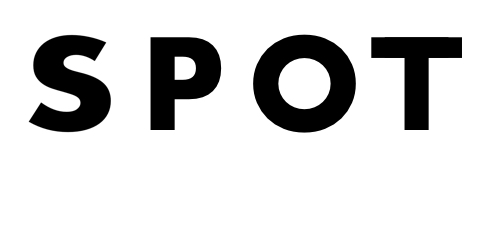
\includegraphics[width=0.6\linewidth]{figures/spot.pdf}
        \caption{%
            Time evolution of a Gaussian absorption line on a rigidly rotating, spotted star computed from the analytic formulae in \S\ref{sec:kT}.
            The stellar surface is modeled as a spherical harmonic expansion up to $l_\mathrm{max}=20$, and the line shape is assumed to be the same everywhere;
            the spot simply downweights the local intensity at all wavelengths.
            As the spot rotates into view (left panel), the line shape changes slightly (center panel). 
            The residuals between the line when the spot is in view (solid) and when it is on the backside of the star (dotted) are shown in the right panel, where a Gaussian-like feature can be seen tracking the spot as it rotates from the blueshifted hemisphere to the redshifted hemisphere of the star.
        }
        \label{fig:spot}
    \end{centering}
\end{figure}

Figure~\ref{fig:compare} shows one of the spectra in Figure~\ref{fig:spot}, this time computed using both our formulae (blue line) and the traditional technique of discretizing the stellar surface, Doppler-shifting the spectrum in each grid cell according to the local radial velocity, interpolating back to a uniform wavelength grid, and summing over the spatial dimension (dotted orange line). 
We show the residuals in the lower panel, where it is clear that as the number of grid cells increases from $10^2$ (light grey) to $10^5$ (dark grey), the numerical solution approaches the solution obtained using our approach.

%Understand---and comment on---the fundamental
%differences between a discrete linear convolution and traditional linear 
%interpolation. 
%Should we expect the numerical solution to actually \emph{converge}
%to the \starry solution, or is the way the two are interpolating fundamentally
%different?

\begin{figure}[t!]
    \begin{centering}
        \includegraphics[width=0.65\linewidth]{figures/compare.pdf}
        \caption{%
            The observed spectrum when the spot is in view computed with our algorithm (blue) and numerically (orange). 
            The problem setup is the same as that in Figure~\ref{fig:spot}. 
            The bottom panel shows the absolute value of the difference between the two spectra for different number of grid points in the numerical solution.
            As the number of grid points increases, the numerical solution approaches the \starry solution.
        }
        \label{fig:compare}
    \end{centering}
\end{figure}

\section{The forward problem}
\label{sec:linear}

\begin{figure}[ht!]
    \begin{centering}
        \includegraphics[width=0.8\linewidth]{figures/linalg.pdf}
        \caption{%
            The Doppler design matrix $\Doppler$ (Equation~\ref{eq:linear:f}), constructed from a grid of Toeplitz matrices, each of shape $K \times K'$, where $K$ is the number of wavelength bins in the broadened spectrum and $K' = K + W - 1$ is the number of bins in the latent (template) spectrum, where $W$ is the width of the convolution kernel.
            The $N$ columns of $\Doppler$ correspond to the Toeplitz matrices for each of the $N$ spherical harmonics (shown at the top);
            the $M$ rows correspond to the Toeplitz matrices rotated to each of the $M$ stellar phases observed (indicated graphically to the left of $\Doppler$).
            The color scale ranges from black (negative) to bright yellow (positive); light grey regions correspond to entries in the matrix that are identically zero.
        }
        \label{fig:linalg}
    \end{centering}
\end{figure}

Although the convolution operator (Equation~\ref{eq:deconv:convolution_def}) is defined for continuous functions, the problem of Doppler imaging deals with discrete measurements of a spectrum in bins of log wavelength. 
Provided our wavelength grid is fine enough, we may therefore approximate Equation~(\ref{eq:deconv:convolution_def}) with a discrete convolution.
For discrete arrays $\bvec{g}$ and $\bvec{h}$, we have
%
\begin{align}
    \label{eq:linear:convolution_def}
    \bvec{g} * \bvec{h} = \bvec{T(g)} \, \bvec{h}
\end{align}
%
where $\bvec{T}$ is a Toeplitz matrix, a matrix whose diagonals are constant from top left to bottom right. 
In this case, the diagonals are constructed from the values of $\bvec{g}$. 
If $\bvec{g}$ has length $L$, element $g_n$ is placed everywhere along the $k^\mathrm{th}$ diagonal of $\bvec{T}$ for $k = -L / 2 + n$; all other entries of $\bvec{T}$ are set to zero. 
Note that the matrix $\bvec{T}$ need not be square; in fact, for our purposes, it is a $(K \times K')$ matrix, where $K$ is the size of the output wavelength grid and $K' = K + W - 1$ is the size of the input wavelength grid (in the rest frame), where $W$ is the width of the convolution kernel.

Given this formulation, we may re-write Equation~(\ref{eq:deconv:F}) as a purely linear operation on $\alm(\lnlam_0)$:
%
\begin{align}
    \label{eq:linear:ft}
    \bvec{f}_m
     & =
    \Doppler_m
    \,
    \alm
    \quad,
\end{align}
%
where $\Doppler_m$ is a $(K \times N K')$ matrix constructed by horizontally concatenating the Toeplitz matrices for each of the $N$ components of the convolution kernel $\kT(\lnlam)$ transformed by the rotation matrix $\bvec{R}(t)$ evaluated at time $t = t_m$:
%
\begin{align}
    \label{eq:linear:Dm}
    \Doppler_m =
    \begin{pmatrix}
        \bvec{T}(\kT_0)
        \quad
         &
        \quad
        \bvec{T}(\kT_1)
        \quad
         &
        \quad
        \cdots
        \quad
         &
        \quad
        \bvec{T}(\kT_N)
        \quad
    \end{pmatrix}
    (\bvec{R}(t_m) \otimes \bvec{I}_{K'})
    \quad.
\end{align}
%
where $\bvec{I}_{K'}$ is the $(K' \times K')$ identity matrix and $\otimes$ denotes the Kronecker product.
%
The $(K \times 1)$ vector $\mathbf{f}_m$ is the model for the flux observed at each wavelength at time $t = t_m$, and the $(N K' \times 1)$ vector $\alm$ is the vector representation of the spatially-dependent spectrum of the star. 
The latter is constructed by flattening the spherical harmonic expansion of the star such that the first $K'$ terms in $\alm$ correspond to the the values of $a_{0,0}$ at each wavelength $\lnlam_0$, followed by the values of $a_{1,-1}$ at each wavelength, and so forth.

In general, our data will consist of observations made at several epochs, corresponding to different rotational phases of the star.
If we concatenate all $M$ spectra $\bvec{f}_m$ into the $(MK \times 1)$ vector $\bvec{f}$, we may write
%
\begin{align}
    \label{eq:linear:f}
    \bvec{f}
     & =
    \Doppler
    \,
    \alm
    \quad,
\end{align}
%
where $\Doppler$ is the full $(MK \times N K')$ Doppler design matrix, constructed by vertically concatenating the individual matrices $\Doppler_m$:
%
%
\begin{align}
    \label{eq:linear:D}
    \Doppler =
    \begin{pmatrix}
        \Doppler_0
        \\
        \Doppler_1
        \\
        \cdots
        \\
        \Doppler_m
    \end{pmatrix}
    \quad.
\end{align}
%
%
Equation~(\ref{eq:linear:f}) represents the full linearization of the problem, where we have expressed the quantity we can observe, $\bvec{f}$, as a linear operation on the quantity of interest, the spectral/spatial decomposition of the stellar surface, $\alm$. 
Figure~\ref{fig:linalg} shows an example of $\Doppler$.
Note, importantly, that this expression does not account for limb darkening or for the fact that spectra are often normalized to the continuum level; we account for these two effects in \S\ref{sec:norm} and \S\ref{sec:ld} below.

\section{The inverse problem}
\label{sec:inverse}
%
In the previous section we showed how to express the data vector $\bvec{f}$, a series of spectra obtained at different epochs, as a purely linear operation on the map vector $\alm$, the spherical harmonic decomposition of the specific intensity on the surface of the star. 
The advantage of this linearity is that, given suitable priors, it allows one to compute both the maximum likelihood solution for $\alm$ and its uncertainty \emph{analytically}. 
In particular, if one places a (multidimensional) Gaussian prior on $\alm$ with mean $\boldsymbol{\mu}_\mathbf{a}$ and covariance $\boldsymbol{\Lambda}_\mathbf{a}$, the maximum \emph{a posteriori} (MAP) solution for $\alm$ is given by the solution to the L2 regularization problem \citep[see, e.g.,][]{Luger2016}:
%
\begin{align}
    \label{eq:inverse:ahat}
    \bvec{\hat{a}} & =
    \boldsymbol{\Sigma}_\mathbf{\hat{a}}
    \left(
    \Doppler^\top
    {\boldsymbol{\Sigma}_\mathbf{f}}^{-1}
    \bvec{f}
    +
    {\boldsymbol{\Lambda}_{\alm}}^{-1} \boldsymbol{\mu}_\mathbf{a}
    \right)
    \quad,
\end{align}
%
with posterior covariance given by
%
\begin{align}
    \label{eq:inverse:acov}
    \boldsymbol{\Sigma}_\mathbf{\hat{a}} & =
    \left(
    \Doppler^\top
    {\boldsymbol{\Sigma}_\mathbf{f}}^{-1}
    \Doppler
    +
    {\boldsymbol{\Lambda}_{\alm}}^{-1}
    \right)^{-1}
    \quad,
\end{align}
%
where $\boldsymbol{\Sigma}_\mathbf{f}$ is the data covariance matrix. 
These equations require the inversion of a few fairly large matrices, but as we will see later, it allows one to obtain the map of the star ($\bvec{\hat{a}}$) and its uncertainty ($\boldsymbol{\Sigma}_{\mathbf{\hat{a}}}$) in under a second for a typical dataset.

There is, however, a catch: for most practical purposes, it is difficult to find a good Gaussian prior for $\bvec{a}$. 
Usually we will have some prior information on what the spectrum of the star is, and perhaps some prior information on the distribution of surface features such as starspots. 
The problem is that even if these priors are Gaussian, the corresponding prior on $\bvec{a}$ is \emph{not}. 
To understand this, consider the case where the stellar rest frame spectrum is spatially constant, save for an amplitude that is spatially variable. 
We can then describe the rest frame spectrum by the $(K' \times 1)$ vector $\bvec{s}$ and the amplitude by the $(N \times 1)$ vector $\bvec{y}$ representing the spherical harmonic expansion of the intensity profile of the star. 
The vector $\alm$ is then given by the (flattened) outer product of the two vectors:
%
\begin{align}
    \label{eq:inverse:alm}
    \alm & = \mathrm{vec}\left( \bvec{A} \right) \nonumber             \\
           & = \mathrm{vec}\left( \bvec{s} \, \bvec{y}^\top \right) \quad,
\end{align}
%
where $\mathrm{vec}$ denotes the vectorization operation, which in this case transforms the $(K' \times N)$ matrix $\bvec{A}$ into the $(N K' \times 1)$ column vector $\alm$ by vertically stacking all of its columns. 
In other words, the vector $\alm$ consists of the set of $K'$ intensities in each wavelength bin repeated $N$ times, each time multiplied by the $n^\mathrm{th}$ spherical harmonic coefficient in the expansion of the surface intensity. 
Returning to our point about priors, note that all of the entries of $\alm$ are the product of two independent random variables. 
Since the product of two random variables is generally non-Gaussian, even when the variables themselves are Gaussian%
\footnote{see, e.g., \url{http://mathworld.wolfram.com/NormalProductDistribution.html}}%
, so too is the prior on $\alm$. 
This point makes Equation~(\ref{eq:inverse:ahat}) tricky to use in practice, since a multivariate Gaussian is not generally the most suitable prior for $\alm$.

That said, a Gaussian prior \emph{is} typically suitable for both the spectrum $\bvec{s}$ and the intensity $\bvec{y}$ (just not their product). 
Spectral templates can provide us with a physically-motivated mean for the prior on $\bvec{s}$, while the variance can be used to capture our degree of confidence in the model.
Similarly, a multivariate Gaussian prior on the spherical harmonic coefficients $\bvec{y}$ is flexible enough to capture prior information on the location and properties of starspots \citep{Luger2021b}.
%
Given Gaussian priors on these two quantities, it is straightforward to show that because Equation~(\ref{eq:linear:f}) is linear in $\alm$, it is also linear in both $\bvec{s}$ and $\bvec{y}$, so MAP solutions can be found analytically for $\bvec{s}$ (conditioned on $\bvec{y}$) and $\bvec{y}$ (conditioned on $\bvec{s}$).
A solution to the full problem of determining both $\bvec{s}$ and $\bvec{y}$ can then be obtained by iteratively solving these two problems.
We investigate this procedure below.

\subsection{Solution for the map}
\label{sec:solve_y}
%
Given a single rest-frame spectrum $\bvec{s}$, the model for the flux vector may be written as
%
\begin{align}
    \label{eq:inverse:fy}
    \bvec{f}
     & =
    \Doppler
    \,
    \bvec{S}
    \,
    \bvec{y}
    \quad,
\end{align}
%
where
%
\begin{align}
    \label{eq:inverse:S}
    \bvec{S} =
    \begin{pmatrix}
        \quadquad\bvec{s}\quadquad &                            &                            &                            &        \\
                                   & \quadquad\bvec{s}\quadquad &                            &                            &        \\
                                   &                            & \quadquad\bvec{s}\quadquad &                            &        \\
                                   &                            &                            & \quadquad\bvec{s}\quadquad &        \\
                                   &                            &                            &                            & \ddots
    \end{pmatrix}
\end{align}
%
is a $(NK' \times N)$ block matrix constructed by repeating the column vector $\bvec{s}$ $N$ times in blocks along the main diagonal.
%
Given prior mean $\boldsymbol{\mu}_\bvec{y}$ and covariance $\boldsymbol{\Lambda}_\bvec{y}$ on $\bvec{y}$, the MAP solution is given by
%
\begin{align}
    \label{eq:inverse:y1hat}
    \bvec{\hat{y}} & =
    \boldsymbol{\Sigma}_\mathbf{\hat{y}}
    \left(
    \bvec{S}^\top\Doppler^\top
    {\boldsymbol{\Sigma}_\mathbf{f}}^{-1}
    \bvec{f}
    +
    {\boldsymbol{\Lambda}_\bvec{y}}^{-1} \boldsymbol{\mu}_\bvec{y}
    \right)
    \quad,
\end{align}
%
with covariance
%
\begin{align}
    \label{eq:inverse:y1cov}
    \boldsymbol{\Sigma}_\bvec{\hat{y}} & =
    \left(
    \bvec{S}^\top\Doppler^\top
    {\boldsymbol{\Sigma}_\bvec{f}}^{-1}
    \Doppler\bvec{S}
    +
    {\boldsymbol{\Lambda}_\bvec{y}}^{-1}
    \right)^{-1}
    \quad.
\end{align}
%
If we choose a prior with diagonal covariance that is constant for each spherical harmonic order $m$,
%
\begin{align}
    \boldsymbol{\Lambda}_\bvec{y} & =
    \mathrm{diag} \left(
    \sigma_0^2
    \quad\quad\quad\quad
    \sigma_1^2
    \quad\quad\quad\quad
    \sigma_1^2
    \quad\quad\quad\quad
    \sigma_1^2
    \quad\quad\quad\quad
    \sigma_2^2
    \quad\quad\quad\quad
    \sigma_2^2
    \quad\quad\quad\quad
    \sigma_2^2
    \quad\quad\quad\quad
    \sigma_2^2
    \quad\quad\quad\quad
    \sigma_2^2
    \quad\quad\quad\quad
    \cdots
    \right)
    \quad,
\end{align}
%
we are in fact imposing an isotropic prior with an angular power spectrum given by $C_l = \sigma_l^2$
\citep[e.g.,][]{Baldi2006}. 
This is especially useful if the typical angular scale of features on the surface of the star is known or if a Gaussian prior can be placed on it.
Alternatively, we may compute $\boldsymbol{\Lambda}_\bvec{y}$ from the Gaussian process formalism in \citet{Luger2021b} to incorporate explicit prior information on the typical latitudes, sizes, and contrasts of spots.
We discuss this point further in \S\ref{sec:discussion:priors}.

\subsection{Solution for the spectrum}
\label{sec:solve_s}
%
Conversely, given a spatial representation of the surface $\bvec{y}$, the model for the flux vector may be written in terms of the spectrum $\bvec{s}$ as
%
\begin{align}
    \label{eq:inverse:fs}
    \bvec{f}
     & =
    \Doppler
    \,
    \bvec{Y}
    \,
    \bvec{s}
    \quad,
\end{align}
%
where
%
\begin{align}
    \label{eq:inverse:Y}
    \bvec{Y} =
    \begin{pmatrix}
        y_{0,0}\, \bvec{I}_{K'} \\
        y_{1,-1}\, \bvec{I}_{K'} \\
        y_{1,0}\, \bvec{I}_{K'} \\
        y_{1,1}\, \bvec{I}_{K'} \\
        \cdots
    \end{pmatrix}
\end{align}
%
is a $(NK' \times K')$ matrix constructed by vertically stacking $N$ $(K' \times K')$ identity matrices, each multiplied by the corresponding coefficient of $\bvec{y}$. 
Given prior mean $\boldsymbol{\mu}_\mathbf{s}$ and covariance $\boldsymbol{\Lambda}_\mathbf{s}$ on $\mathbf{s}$, the MAP solution is given by
%
\begin{align}
    \label{eq:inverse:shat}
    \bvec{\hat{s}} & =
    \boldsymbol{\Sigma}_\mathbf{\hat{s}}
    \left(
    \bvec{Y}^\top\Doppler^\top
    {\boldsymbol{\Sigma}_\mathbf{f}}^{-1}
    \bvec{f}
    +
    {\boldsymbol{\Lambda}_\mathbf{s}}^{-1} \boldsymbol{\mu}_\mathbf{s}
    \right)
    \quad,
\end{align}
%
with covariance
%
\begin{align}
    \label{eq:inverse:scov}
    \boldsymbol{\Sigma}_\mathbf{\hat{s}} & =
    \left(
    \bvec{Y}^\top\Doppler^\top
    {\boldsymbol{\Sigma}_\mathbf{f}}^{-1}
    \Doppler\bvec{Y}
    +
    {\boldsymbol{\Lambda}_\mathbf{s}}^{-1}
    \right)^{-1}
    \quad.
\end{align}

\subsection{The full solution}
\label{sec:full_solve}
%
In the previous two sections we showed how, if the stellar rest-frame spectrum is spatially constant and known \emph{a priori} (from, say, a template spectrum), the posterior distribution for the surface map $\bvec{y}$ is \emph{analytic} (Equations~\ref{eq:inverse:y1hat} and \ref{eq:inverse:y1cov}). 
Conversely, if the surface map is known, the posterior for the spectrum is also analytic (Equations~\ref{eq:inverse:shat} and \ref{eq:inverse:scov}). 
Both sets of solutions require Gaussian priors on the quantities of interest, but these are easily interpretable. 
A Gaussian prior on the spherical harmonic coefficients of the surface map corresponds to the angular power spectrum of the surface features, whereas a Gaussian prior on the spectrum can be used to correctly propagate uncertainties in the stellar spectrum from observational uncertainties on the stellar metallicity, temperature, etc.

Importantly, the framework developed here allows one to analytically compute not only the ``optimal'' solution to the Doppler imaging problem, but also its uncertainty. 
The problem of re-constructing surface images of stars from spectra and/or light curves is fundamentally ill-posed because of intrinsic degeneracies and a large null space \citep[e.g.,][]{Cowan2017,Luger2019,Luger2021a}. 
Coupled to uncertainties in properties like the stellar inclination, rotation period, and limb darkening coefficients, as well as the finite signal-to-noise ratio of the data, this makes the process of searching for the ``optimal'' solution flawed at best, and meaningless at worst. 
Access to the full covariance matrix of the solution is therefore essential to assessing our confidence in the various features of the inferred surface maps.

However, as we mentioned above, the Doppler imaging problem can be solved analytically for either the surface map or the spectrum, but not typically both. 
If neither are known exactly \emph{a priori}, which is quite often the case, we can still find the MAP solution quickly by guessing at an initial spectrum $\bvec{s}$ and iterating between optimizing for $\bvec{y}$ and optimizing for $\bvec{s}$. 
Note, importantly, that this bilinear problem is not generally convex: the likelihood space often has many local minima, which can in principle make it difficult to find the true solution.
Nevertheless, given a good starting point for $\bvec{s}$ and sufficient regularization on $\bvec{y}$, we find that it typically converges to the correct solution; see \S\ref{sec:spotstar}.

Once the MAP solution has been found for both $\bvec{s}$ and $\bvec{y}$, the covariance of one conditioned on the other can be computed from the formulae above. 
However, this is necessarily a lower bound on the true covariance of the solution, since it neglects any covariance \emph{between} $\bvec{s}$ and $\bvec{y}$. 
To \emph{correctly} account for this, one must resort to Monte Carlo methods or other sampling techniques. 
We discuss this further in \S\ref{sec:discussion:priors}.

\section{Further considerations}
\label{sec:bellswhistles}
%
Before we demonstrate our formalism in practice, we consider three modifications to our model that are often required when modeling real data. 
Below we discuss what to do when the relative brightness of the star across different observations is unknown (\S\ref{sec:norm}), how to account for the effects of limb darkening (\S\ref{sec:ld}), and how to model stars whose local spectra differ within and outside of starspots (\S\ref{sec:eigen}).

\subsection{Unknown continuum normalization}
\label{sec:norm}
%
Consider the star depicted in Figure~\ref{fig:spot}. 
When the spot is in view, absorption lines become distorted due to the suppression of either blueshifted or redshifted light. 
However, what is not shown in the figure is the fact that overall, the star also gets \emph{dimmer}: the continuum level drops in the presence of the spot. 
Unfortunately, spectrographs are not usually designed to measure this, since the change in the star's overall brightness from one observation to the next is often dwarfed by (unknown) changes in the spectrograph sensitivity, cloud cover, etc.
For this reason, the spectra are usually normalized to have a fixed baseline continuum, and Equation~\ref{eq:linear:f} is no longer a good model for the data.

One option is to collect simultaneous photometry on the target in a band similar to the wavelength range observed, and use this light curve to (un-)normalize the spectral timeseries $\bvec{f}$. 
However, when this is not an option, our model for $\bvec{f}$ (Equation~\ref{eq:linear:f}) must be amended:
%
\begin{align}
    \label{eq:norm:f}
    \fnorm
     & =
     \frac{
        \mathbf{f}
    } {
        \bvec{B}
        \,
        \alm
    }
    \nonumber 
    \\[1em]
    & =
    \frac{
        \Doppler
        \,
        \alm
    } {
        \bvec{B}
        \,
        \alm
    }
    \quad,
\end{align}
%
where $\fnorm$ is the normalized spectral timeseries, $\bvec{B}$ is the baseline design matrix, and the vector division is performed elementwise. 
If $c$ is an index in the observed spectrum corresponding to the continuum (at all epochs), the elements of $\bvec{B}$ are computed from
%
\begin{align}
    B_{ij} = D_{i'j}
\end{align}
%
where
%
\begin{align}
    i' = c + \bigg\lfloor\frac{i}{K}\bigg\rfloor K
    \quad.
\end{align}
%
In other words, the matrix $\bvec{B}$ is constructed by repeating the $c^\mathrm{th}$ row of each epoch block $\Doppler_m$ of $\Doppler$ $K$ times.
Equation~(\ref{eq:norm:f}) is therefore equivalent to computing the $M$ unnormalized spectra using Equation~(\ref{eq:linear:f}) and dividing each one by the value at index $c$.


Given this new equation, we must change how we approach the inverse problem (\S\ref{sec:inverse}) if our data vector is the normalized spectral timeseries $\fnorm$. 
When solving for the spectrum given the spherical harmonic vector (\S\ref{sec:solve_s}), we need only make the replacements 
%
$\bvec{f} \rightarrow \fnorm \circ (\bvec{B}\, \bvec{a})$ 
%
and 
%
$\boldsymbol{\Sigma}_\mathbf{f} \rightarrow \boldsymbol{\Sigma}_{\fnorm} \circ (\bvec{B}\, \bvec{a})^2$ 
%
in Equations~(\ref{eq:inverse:shat}) and (\ref{eq:inverse:scov}), where $\circ$ denotes the elementwise product.
However, when solving for the spherical harmonic vector given the spectrum (\ref{sec:solve_y}), the problem is no longer linear in $\bvec{y}$, as the vector of interest appears in both the numerator and the denominator:
%
\begin{align}
    \label{eq:norm:fy}
    \fnorm
     & =
    \frac{
        \bvec{D}
        \,
        \bvec{S}
        \,
        \bvec{y}
    }{
        \bvec{B}
        \,
        \bvec{S}
        \,
        \bvec{y}
    }
    \quad.
\end{align}
%
Unfortunately, this equation does not admit a closed form solution for $\mathbf{y}$. 
One can, however, still solve for the maximum a posteriori value of $\mathbf{y}$ in an efficient manner by iteratively solving for the baseline and then for the spherical harmonic coefficients.
We describe a procedure for this in \S\ref{sec:spotstar} below.

\subsection{Limb darkening}
\label{sec:ld}
%
Thus far we have avoided mention of limb darkening, whose effect on the observed spectrum can often be significant. 
A proper treatment of limb darkening requires solution of radiative transfer equations and should account for the temperature and composition gradients in the stellar atmosphere. 
However, in the spirit of data-driven inference, we can approximate the effect of limb darkening by weighting the spatial component of our map by the limb darkening profile of the star, which can either be imposed or learned from the data. 
For a polynomial limb darkening law of the form
%
\begin{align}
    \label{eq:ld:I}
    \frac{I(\mu)}{I(\mu = 1)} = 1 - \sum_{n=1}^{n_\mathrm{max}} u_n(1 - \mu)^n
    \quad,
\end{align}
%
where $\mu = z = \sqrt{1 - x^2 - y^2}$ is the radial coordinate on the projected disk and $u_n$ is a limb darkening coefficient, the effect of limb darkening on the stellar map can be expressed exactly as a linear operation on the spherical harmonic coefficient vector \citep{Luger2019,Agol2020}. 
This can be understood by noting that all terms in Equation~(\ref{eq:ld:I}) are strictly polynomials in $x$, $y$, and $z$, all of which can be expressed exactly as sums of spherical harmonics \citep{Luger2019}. 
When weighting the surface intensity by the limb darkening profile, the resulting intensity is simply a product of spherical harmonics, which is itself a sum of spherical harmonics. 
Given a limb darkening law of degree $n_\mathrm{max}$, we can always construct a matrix $\bvec{L}$ that transforms a spherical harmonic vector $\bvec{y}$ of degree $l_\mathrm{max}$ to a limb-darkened spherical harmonic vector $\bvec{y'}$ of degree $l_\mathrm{max} + n_\mathrm{max}$. 
As an example, consider a map of degree $l_\mathrm{max} = 1$ and the linear limb darkening law ($n_\mathrm{max} = 1$).
The transformation matrix from $\bvec{y}$ to $\bvec{y'}$ is
%
\begin{align}
    \label{eq:ld:L}
    \bvec{L} =
    \frac{1}{1 - \frac{u_1}{3}}
    \begin{pmatrix}
        \quadquad1-u_1\quadquad & 0                       & \frac{u_1}{\sqrt{3}}    & 0                       \\
        0                       & \quadquad1-u_1\quadquad & 0                       & 0                       \\
        \frac{u_1}{\sqrt{3}}    & 0                       & \quadquad1-u_1\quadquad & 0                       \\
        0                       & 0                       & 0                       & \quadquad1-u_1\quadquad \\
        0                       & 0                       & 0                       & 0                       \\
        0                       & \frac{u_1}{\sqrt{5}}    & 0                       & 0                       \\
        0                       & 0                       & \frac{2u_1}{\sqrt{15}}  & 0                       \\
        0                       & 0                       & 0                       & \frac{u_1}{\sqrt{5}}    \\
        0                       & 0                       & 0                       & 0
    \end{pmatrix}
    \quad.
\end{align}
%
The columns of $\bvec{L}$ are constructed from the coefficient vectors of each transformed spherical harmonic, which are in turn computed by multiplying each spherical harmonic by the spherical harmonic decomposition of the particular limb darkening law.
Figure~\ref{fig:ld} shows this transformation with $u_1 = 1$ applied to each of the first four spherical harmonics.
%
\begin{figure}[t!]
    \begin{centering}
        \includegraphics[width=0.5\linewidth]{figures/ld.pdf}
        \caption{%
            Illustration of the limb darkening transformation given by Equation~(\ref{eq:ld:L}) for a linear limb darkening law with $u_1 = 1$. 
            Each row shows a spherical harmonic before (left) and after (right) transformation by $\bvec{L}$.
        }
        \label{fig:ld}
    \end{centering}
\end{figure}
%

Now, to incorporate limb darkening into our model, we must modify how we compute the Doppler design matrix $\Doppler$ (Equation~\ref{eq:linear:D} and Figure~\ref{fig:linalg}). 
Recall that this matrix is constructed by vertically stacking the submatrices $\Doppler_m$ given by Equation~(\ref{eq:linear:Dm}), which we now compute as
%
\begin{align}
    \label{eq:ld:Dm}
    \Doppler_m =
    \begin{pmatrix}
        \quad
        \bvec{T}(\kT_0)
        \quad
         &
        \quad
        \bvec{T}(\kT_1)
        \quad
         &
        \quad
        \cdots
        \quad
         &
        \quad
        \bvec{T}(\kT_{N'})
        \quad
    \end{pmatrix}
    (\bvec{L} \, \bvec{R}(t_m) \otimes \bvec{I}_{K'})
    \quad,
\end{align}
%
where we have replaced the rotation matrix $\bvec{R}(t_m)$ with the linear transformation $\bvec{L}\,\bvec{R}(t_m)$, which first rotates the input spherical harmonic coefficient vector to the correct phase then limb darkens it. 
Note also that the terms in the convolution kernel $\kT$ are now indexed from 0 to $N' = (l_\mathrm{max} + n_\mathrm{max} + 1)^2$, where $n_\mathrm{max}$ is the degree of the limb darkening operator.

Note that it is also possible to model wavelength-dependent limb darkening in this fashion. 
The procedure is similar, except that the limb darkening coefficients $u_n$ are now functions of $\lnlam$, and each element of the matrix $\bvec{L}$ is now a vector of length $K'$. 
The submatrices $\Doppler_m$ may be written as
%
\begin{align}
    \label{eq:ld:Dmwav}
    \resizebox{0.91\textwidth}{!}{
        $
            \Doppler_m =
            \begin{pmatrix}
                \quad
                \bvec{T}(\kT_0)
                \quad
                 &
                \quad
                \bvec{T}(\kT_1)
                \quad
                 &
                \quad
                \cdots
                \quad
                 &
                \quad
                \bvec{T}(\kT_{N'})
                \quad
            \end{pmatrix}
            \begin{pmatrix}
                \mathrm{diag}(\bvec{L}_{0,0})
                 &
                \mathrm{diag}(\bvec{L}_{0,1})
                 &
                \cdots
                 &
                \mathrm{diag}(\bvec{L}_{0,N})
                \\
                \mathrm{diag}(\bvec{L}_{1,0})
                 &
                \mathrm{diag}(\bvec{L}_{1,1})
                 &
                \cdots
                 &
                \mathrm{diag}(\bvec{L}_{1,N})
                \\
                \cdots
                 &
                \cdots
                 &
                \ddots
                 &
                \cdots
                \\
                \mathrm{diag}(\bvec{L}_{N',0})
                 &
                \mathrm{diag}(\bvec{L}_{N',1})
                 &
                \cdots
                 &
                \mathrm{diag}(\bvec{L}_{N',N})
            \end{pmatrix}
            (\bvec{R}(t_m) \otimes \bvec{I}_{K'})
        $
    }
    \quad,
\end{align}
%
where $\mathrm{diag}(\bvec{v})$ denotes the $(K' \times K')$ diagonal matrix constructed by placing the vector $\bvec{v}$ along the main diagonal.

\subsection{Multiple spectral components}
\label{sec:eigen}
%
In our discussion so far we have focused on the particular case where the spectral/spatial decomposition of the stellar surface can be expressed as the outer product of two vectors (Equation~\ref{eq:inverse:alm}). 
As we mentioned previously, this corresponds to the case where the spectrum is constant across the surface of the star except for a spatially-variable amplitude: i.e., spots have the same spectrum as the rest of the star, but emit less flux overall. 
However, most of the formalism developed here also applies to the more general case where the spectrum at a particular point on the surface of the star is a linear combination of several different spectral components. 
In this case, the map vector $\alm$ may be written as the sum over $J$ spectra $\bvec{s}_j$, each of which is dotted into a different vector of spherical harmonic coefficients $\bvec{y}_j^\top$:
%
\begin{align}
    \label{eq:eigen:alm}
    \alm
     & =
    \sum_{j=0}^{J-1}\mathrm{vec}\left( \bvec{s}_j \, \bvec{y}_j^\top \right) \\
     & =
    \mathrm{vec}\left( \boldsymbol{\mathbb{S}} \, \boldsymbol{\mathbb{Y}}^\top \right) \quad,
\end{align}
%
where $\boldsymbol{\mathbb{S}}$ is the $(K' \times J)$ matrix whose columns are the $J$ spectral components and $\boldsymbol{\mathbb{Y}}^\top$ is the $(J \times N)$ matrix whose rows are the corresponding $J$ spherical harmonic coefficient vectors.

The model remains linear in both the spherical harmonic coefficients and the spectral components, and the procedures outlined in \S\ref{sec:inverse} may still be followed to solve the inverse problem, provided we unroll these matrices into vectors, letting $\mathbf{s} = \mathrm{vec}(\boldsymbol{\mathbb{S}})$ and $\mathbf{y} = \mathrm{vec}(\boldsymbol{\mathbb{Y}})$.
We present an example of inference on a two-component stellar spectrum in \S\ref{sec:twospec} below.

\section{Application to a spotted star}
\label{sec:spotstar}

In this section we apply the formalism developed in \S\ref{sec:inverse} and \S\ref{sec:bellswhistles} to a synthetic dataset of a rapidly rotating spotted star. 
This section is motivated by the examples in \cite{Vogt1987}, who generated rotationally-broadened spectra of a rapidly-rotating star with the letters ``VOGT'' painted across the northern hemisphere. 
In that paper, the authors generated synthetic line profiles of the Fe I $\lambda 6430$ absorption line with equivalent width ${\sim}10$~km/s and from these computed rotationally broadened spectra for a star at an inclination $i=40^\circ$ rotating at projected velocity $v\sin i = 40$~km/s.
The spectra were computed at 16 equally spaced rotational phases and downsampled to 32 wavelength bins per epoch, for a total of 512 data points.

\begin{figure}[t!]
    \begin{centering}
        \includegraphics[width=0.85\linewidth]{figures/spot_setup.pdf}
        \caption{%
            The basic setup for the \spot problem. 
            We compute the $l_\mathrm{max} = 15$ spherical harmonic expansion of a map where the word ``SPOT'' has been placed across the northern hemisphere (top left). 
            Each point on the surface is given the same spectrum, composed of a sum of synthetic Gaussian absorption lines (blue curve in the bottom panel).
            The specific intensity at each point on the surface is equal to this spectrum weighted by the intensity of the map, which is close to zero within the spot (point labeled \texttt{B}) and close to unity outside the spot (point labeled \texttt{A}).
            To generate the synthetic dataset (orange curves in the bottom panel), the star is inclined at $40^\circ$ with respect to the line of sight and the disk-integrated spectrum is computed at 16 equally-spaced phases between $-180^\circ$ and $180^\circ$, assuming an equatorial velocity $v = 60$ km/s (middle panel).
            The grey regions indicate wavelength regions outside the observation window, but whose features can still contribute to the observed spectrum due to rotational broadening.
        }
        \label{fig:spot_setup}
    \end{centering}
\end{figure}

We repeat the same experiment here using our new formalism, except we instead generate a stellar surface with the word ``SPOT'' written across the northern hemisphere (top left panel of Figure~\ref{fig:spot_setup}).
We do this by computing the $l_\mathrm{max} = 15$ spherical harmonic decomposition of an image of the word, generating a set of $N = (l_\mathrm{max} + 1)^2 = 256$ spherical harmonic coefficients $\bvec{y}$. 
We assume an equatorial velocity $v = 60$ km/s and an inclination $i = 40^\circ$, such that $v \sin i = 38.6$~km/s (compare to $i = 40^\circ$ and $v \sin i = 40$~km/s in \citealt{Vogt1987}).

Our input spectrum $\bvec{s}$ was generated at extremely high resolution
%
($R \equiv \frac{\lambda}{\Delta\lambda} = 750,000$) 
%
centered on the Fe I $\lambda 6430$ absorption line (blue curve in the bottom panel of Figure~\ref{fig:spot_setup}).
%
The spectrum consists of a (purely synthetic) Gaussian absorption line of fractional depth 50\% centered at $\lambda = 643$~nm with FWHM of $0.02$~nm, or, in velocity space, $\Delta v = \mathrm{FWHM} \times c / \lambda \approx~10$~km/s, equal to the value used in \citet{Vogt1987}. 
%
Unlike \citet{Vogt1987}, we add two additional small absorption lines, one of which is blended with the central absorption line.
In total, the rest frame spectrum $\bvec{s}$ consists of 
%
$K = 351$ 
%
wavelength bins in the range $642.85~\mathrm{nm} \leq \lambda \leq 643.15~\mathrm{nm}$ plus an additional
%
$W - 1 = 252$ 
%
bins of padding 
%
(126 on either side) 
%
to eliminate edge effects due to the convolution, for a total of 
%
$K' = 603$
%
wavelength bins. 
Finally, we linearly interpolate this spectrum to a wavelength grid uniform in log space to obtain the vector $\bvec{s}$ evaluated at each $\lnlam$.

Given $\bvec{y}$ and $\bvec{s}$, we use Equations~(\ref{eq:deconv:F}) and~(\ref{eq:inverse:alm}) to compute the data vector $\bvec{f}$, which we downsample to a grid of 
%
$K_\mathrm{obs} = 70$ 
%
wavelength bins in the range $642.85~\mathrm{nm} \leq \lambda \leq 643.15~\mathrm{nm}$, corresponding to a resolution of
%
$R = 150,000$.
%
We compute $\bvec{f}$ at $M = 16$ equally spaced rotational phases; these phases are shown in orthographic projection (as an observer would see the star) in the center panel of Figure~\ref{fig:spot_setup}. 
The synthetic spectra for each phase are shown as the orange curves in the bottom panel of the figure (note the different scaling, as all spectral lines become shallower due to the broadening). 
%
We assume a wavelength-independent, quadratic limb darkening law with $u_1 = 0.5$ and $u_2 = 0.25$. 
Finally, we divide the flux by the baseline at each epoch (Equation~\ref{eq:norm:f}) and add random Gaussian noise with covariance matrix $\boldsymbol{\Sigma}_\bvec{f} = \sigma_\bvec{f}^2 \mathbf{I}$, with $\sigma_\bvec{f} = 2\times 10^{-4}$ to simulate a very high signal-to-noise ratio (SNR) spectrum. 
The typical fractional line depth in the observed spectrum is 0.2, so our choice of $\sigma_\bvec{f}$ corresponds to SNR $\sim 10^{3}$ in each of the 70 wavelength bins of $\bvec{f}$.

In the following sections we discuss various approaches to solving the Doppler imaging problem for this dataset.
Unless otherwise noted, in all experiments we adopt a Gaussian prior for the spherical harmonic coefficients $\bvec{y}$ with mean $\boldsymbol{\mu}_\bvec{y} = \left(1 \quad\quad \bvec{0}\right)$ and covariance $\boldsymbol{\Lambda}_\bvec{y} = 10^{-4} \bvec{I}$, corresponding to a flat power spectrum prior.
When solving for the rest frame spectrum, we also place a Gaussian prior on $\bvec{s}$ with unit mean and covariance $\boldsymbol{\Lambda}_\bvec{s} = 10^{-3}\bvec{I}$.
These choices are arbitrary and primarily based on trial-and-error given knowledge of the true solutions.
We discuss strategies for choosing optimal priors for real datasets in \S\ref{sec:discussion:priors} below.

\subsection{Known baseline and spectrum}
\label{sec:spot_y1}
%
In our first experiment, we attempt to infer the stellar map assuming we have perfect knowledge of the rest frame spectrum $\bvec{s}$ and the baseline, as well as the stellar inclination, rotation period, and limb darkening coefficients.
This is analogous to the case where a good physical model exists for the stellar spectrum and simultaneous photometry is available to constrain the baseline variations.
As we showed in \S\ref{sec:solve_y}, the posterior distribution for the map coefficients $\bvec{y}$ is analytic in this case, with mean given by Equation~(\ref{eq:inverse:y1hat}) and covariance given by Equation~(\ref{eq:inverse:y1cov}). 
Note that we must first scale the data vector $\fnorm$ by the baseline (which in this case is known) to obtain $\bvec{f}$.

\begin{figure}[p!]
    \begin{centering}
        \includegraphics[width=0.39\linewidth]{figures/spot_infer_y_timeseries.pdf}
        \includegraphics[width=0.59\linewidth]{figures/spot_infer_y_maps.pdf}
        \caption{%
            The solution to the \spot problem at high SNR when both the rest frame spectrum and the baseline are known.
            The panel on the left shows the inferred map at each of the 16 epochs, alongside the observed spectrum (black points) and the best-fit model (orange lines). 
            The Mollweide projection of the original map is shown at the top right; the inferred map is displayed below it. 
            The bottom panel shows the posterior uncertainty on the inferred intensity, ranging from close to zero in the northern hemisphere to $\sigma_\mathrm{prior} \approx 13\%$ below a latitude of $-30^\circ$. 
            The latter is the uncertainty associated with our particular choice of prior, as the southernmost latitudes of the star are never visible to the observer.
            The optimization step in this experiment ran in \timeInferY.
        }
        \label{fig:spot_infer_y}
    \end{centering}
\end{figure}

Figure~\ref{fig:spot_infer_y} shows the results.
The left hand panel shows the inferred map alongside the data (black points) and best fit model (orange curves) at each of the 16 epochs.
The panels on the right show the true map (top), the inferred map (center) and the posterior pointwise uncertainty (bottom) on a Mollweide grid. 
The uncertainty on the vector of pixels $\bvec{p}$ where we evaluate the map is equal to the square root of the diagonal of the posterior covariance matrix for the pixel values, computed from
%
\begin{align}
    \label{eq:spotstar:uncert}
    \boldsymbol{\Sigma}_\bvec{p} = \bvec{P} \boldsymbol{\Sigma}_\bvec{\hat{y}}\bvec{P}^\top
\end{align}
%
where $\bvec{P}$ is the change-of-basis matrix from spherical harmonic coefficients to pixels on the grid.

The inferred map very closely matches the true map, aside from a few small artifacts in the southern hemisphere.
Note, importantly, that regions south of the equator are almost never in view to the observer (below $-40^\circ$, they are \emph{never} in view); our inferred map is therefore informed primarily by our prior in southern latitudes.
This is well captured by the uncertainty (bottom panel), which increases south of the equator, reaching a maximum at $-30^\circ$, below which the uncertainty is constant at about 13\%, a value associated with our particular choice of prior.

\subsection{Known spectrum, unknown baseline}
\label{sec:spot_y1b}
%
We next investigate the case where the spectrum is known exactly, but the baseline is not. 
This corresponds to the case discussed in \S\ref{sec:norm}, in which each spectrum is normalized to its continuum, and the true difference in continuum levels across spectral epochs is not precisely known.
This is likely to be the most common application of the methodology presented in this work.

Our approach is to iteratively solve Equation~(\ref{eq:norm:fy}) by re-expressing it as
%
\begin{align}
    \fnorm
     & =
    \frac{
        \bvec{D}
        \,
        \bvec{S}
        \,
        \bvec{y}
    }{
        \bvec{b}
    }
    \quad.
\end{align}
%
where the baseline $\bvec{b}$ is given by
%
\begin{align}
    \bvec{b}
    =
    \bvec{B}
    \,
    \bvec{S}
    \,
    \bvec{y}
    \quad.
\end{align}
%
We adopt a simple iterative scheme where we solve the L2 problem for $\bvec{y}$ with $\bvec{b}$ fixed, then update the value of $\bvec{b}$ and repeat.
Because of the high SNR of our data, we find that it is necessary to employ a simple tempering procedure, in which we artificially inflate the variance of the data by a factor $T$, which we slowly decrease with each step until $T = 1$. 
This has the effect of smoothing out the likelihood surface, effectively preventing the solver from getting stuck in local minima.
For this particular experiment, we set $\ln T_0 = 2$ and $\Delta \log T = -0.04$, for a total of $50$ steps of the bilinear solver.
We also add a small variance term $\sigma_b^2 = 10^{-2}$ to all entries of the data covariance $\boldsymbol{\Sigma}_{\bvec{f}}$; this has the effect of marginalizing over a small additive model term, which we find improves the convergence of the algorithm.

\begin{figure}[p!]
    \begin{centering}
        \includegraphics[width=0.39\linewidth]{figures/spot_infer_yb_timeseries.pdf}
        \includegraphics[width=0.59\linewidth]{figures/spot_infer_yb_maps.pdf}
        \caption{%
            Similar to Figure~\ref{fig:spot_infer_y}, but assuming the input spectra are continuum-normalized.
            We are able to infer the surface map just as well as in the case where the true continuum level is known (Figure~\ref{fig:spot_infer_y}). 
            As before, regions south of the equator are almost never in view, so that portion of our inferred map is dominated by the prior.
            Note that the uncertainty shown (lower panel) is a strict lower bound on the true uncertainty, as it is conditioned on our point estimate of the baseline level.
            The optimization step in this experiment ran in \timeInferYB.
        }
        \label{fig:spot_infer_yb}
    \end{centering}
\end{figure}

Our results are shown in Figure~\ref{fig:spot_infer_yb}.
As in the case where the continuum level was known exactly (Figure~\ref{fig:spot_infer_y}), we recover the stellar surface map with high fidelity in the northern hemisphere.
However, there is now a strong dipolar artifact; the background intensity level is higher in the northern hemisphere than in the southern hemisphere.
This is due to a degeneracy involving the $Y_{1,-1}$ spherical harmonic (\raisebox{-0.2em}{\includegraphics[width=1em]{figures/Y1m1.pdf}}), which, because a large portion of the southern hemisphere is never in view, cannot be constrained by the data.

Interestingly, while the map uncertainty still increases toward the south pole (bottom panel), its magnitude is smaller than that in Figure~\ref{fig:spot_infer_y}.
This is counter-intuitive, since the continuum-normalized spectrum should contain \emph{less} information than the unnormalized one.
Indeed, the uncertainties shown in the figure are conditioned on our estimate of the baseline, so they are actually a strict \emph{lower bound} on the map uncertainty.
In order to constrain the true uncertainty on the solution to this bilinear problem, we must resort to approximate sampling methods such as MCMC. 
We discuss this further in \S\ref{sec:discussion:priors}.

\subsection{Unknown spectrum, unknown baseline}
\label{sec:spot_y1bs}
%
Suppose we are handed a series of spectra in a wavelength regime where we do not have a good physical model for the line generation mechanisms, or a wavelength regime with many line blends for which we do not have reliable templates. 
Or perhaps the spectra are of a star whose rotational broadening does not dominate over other broadening mechanisms, in which case our template might not be accurate enough to allow us to tease out the small Doppler signals. 
In these cases, we may want to relax the assumption that we know the rest frame spectrum $\bvec{s}$ exactly, and instead try to \emph{learn} it from the data.

Given the same data as before, we now try to learn both the stellar map and the stellar spectrum, conditioned only on the wide Gaussian priors discussed above. 
We must follow the iterative procedure presented in
\S\ref{sec:full_solve}, adjusting for the fact that we do not know the true baseline, either (\S\ref{sec:norm}).

\begin{figure}[p!]
    \begin{centering}
        \includegraphics[width=0.39\linewidth]{figures/spot_infer_ybs_timeseries.pdf}
        \includegraphics[width=0.59\linewidth]{figures/spot_infer_ybs_maps.pdf}
        \vspace{1em}
        \includegraphics[width=\linewidth]{figures/spot_infer_ybs_spectra.pdf}
        \caption{%
            Similar to Figure~\ref{fig:spot_infer_y}, but assuming we have no information about either the spectrum, the baseline, or the map coefficients. 
            The bottommost panel now shows the true rest frame spectrum (blue line), the initial guess based on a deconvolution (dashed orange line), and the inferred spectrum (orange line, with shaded $1\sigma$ uncertainty).
            The optimization step in this experiment ran in \timeInferYBS.
        }
        \label{fig:spot_infer_ybs}
    \end{centering}
\end{figure}

\begin{figure}[p!]
    \begin{centering}
        \includegraphics[width=0.39\linewidth]{figures/spot_infer_ybs_low_snr_timeseries.pdf}
        \includegraphics[width=0.59\linewidth]{figures/spot_infer_ybs_low_snr_maps.pdf}
        \includegraphics[width=\linewidth]{figures/spot_infer_ybs_low_snr_spectra.pdf}
        \caption{%
            Same as Figure~\ref{fig:spot_infer_ybs}, but for $10\times$ lower SNR.
            We still recover the \spot map and the input spectrum, albeit with higher uncertainty, as expected.
            Once again, the optimization step in this experiment ran in \timeInferYBSLOSNR.
        }
        \label{fig:spot_infer_ybs_low_snr}
    \end{centering}
\end{figure}

Because the problem is generally not convex, we need a good starting guess for either the spectrum or the map coefficients. 
We note that we can very crudely approximate the rest frame spectrum by deconvolving the average observed spectrum with the first term of the convolution kernel $\kT$ (\raisebox{-0.1em}{\includegraphics[width=2em]{figures/kT00.pdf}}); we do this by solving the linear problem in Equation~(\ref{eq:linear:convolution_def}) with aggressive regularization.
In practice, this is a fairly poor approximation, but we find that it suffices as an initial guess. 
We then iterate between solving for $\bvec{y}$ (\S\ref{sec:solve_y}) and solving for $\bvec{s}$ (\S\ref{sec:solve_s}), followed by a step in which we update our estimate of the baseline.
We adopt the same tempering scheme discussed above.

Figure~\ref{fig:spot_infer_ybs} shows the results; the top portion of the figure is the same as in Figure~\ref{fig:spot_infer_yb}.
A panel has been added at the bottom showing the true rest frame spectrum (blue), the initial guess based on the deconvolution (dashed orange), and the inferred spectrum with 1-$\sigma$ uncertainty shading (orange). 
We recover the \spot feature as before, albeit with more noise, particularly south of the equator. 
Once again, our map uncertainties are somewhat underestimated, as expected, since they are computed conditioned on the optimum value of the baseline and the spectrum. 
On the other hand, we recover the spectrum exceedingly well, with low uncertainty and virtually no bias anywhere.

To test our technique on more realistic data, we repeat the experiment on data with $10$ times higher uncertainty, setting $\sigma_\bvec{f} = 2\times 10^{-3}$.
%
After some tuning, we find it necessary to increase our prior variances slightly to get good fits to the data: we set $\boldsymbol{\Lambda}_\bvec{y} = 2\times 10^{-4} \bvec{I}$ and $\boldsymbol{\Lambda}_\bvec{s} = 2\times 10^{-2}\bvec{I}$.
%
Figure~\ref{fig:spot_infer_ybs_low_snr} shows the results.
We again correctly infer the \spot feature and the rest frame spectrum, although the surface map is considerably degraded, particularly at high spatial frequencies.

\subsection{Spatially-variable spectrum}
\label{sec:twospec}
%
In our final experiment, we relax the assumption that the stellar rest frame spectrum is spatially constant, allowing for different spectral features inside and outside of the \spot. 
This is the case for, say, chemically peculiar Ap stars, whose abundance of certain elements is significantly different within spotted regions on their surfaces. 
It is also the case in general for spots that are significantly cooler than the rest of the photosphere, where the relative abundance of different ionization states or molecular features may be different than in the hotter, unspotted regions.

The problem setup is the same as that discussed in \S\ref{sec:eigen}, where our full map vector $\bvec{a}$ is the outer product of a spectral matrix $\mathbb{S}$, whose $J$ columns are the different spectral components, and a spherical harmonic coefficient matrix $\mathbb{Y}^\top$, whose $J$ rows are the corresponding coefficient vectors. 
For simplicity, in this experiment we consider only $J = 2$ map components and further require that the surface map for the second component is the complement of the surface map for the first component.
Specifically, the first component map ($\bvec{y_0}$, the first row of $\mathbb{Y}^\top$) corresponds to the background photosphere, whose value is unity everywhere except within the \texttt{SPOT} feature, where the value is zero.
The second component map ($\bvec{y_1}$, the second row of $\mathbb{Y}^\top$) corresponds to the spot and is zero in the photosphere and unity within the spot.
The two columns of $\mathbb{S}$ are $\bvec{s_0}$ and $\bvec{s_1}$, the unknown spectral components corresponding to the photosphere and the spot, repsectively.
%
\begin{figure}[p!]
    \begin{centering}
        \includegraphics[width=0.39\linewidth]{figures/twospec_timeseries.pdf}
        \includegraphics[width=0.59\linewidth]{figures/twospec_maps.pdf}
        \includegraphics[width=\linewidth]{figures/twospec_spectra1.pdf}
        \includegraphics[width=\linewidth]{figures/twospec_spectra2.pdf}
        \caption{%
            An example of a star whose spectrum is different within the spot and outside of the spot.
            We are able to infer both the surface map of the star (upper right) and the two component spectra (lower two panels), assuming virtually no prior knowledge of either.
            The optimization step in this experiment ran in \timeInferTwoSpec.
        }
        \label{fig:twospec}
    \end{centering}
\end{figure}
%
We set $\bvec{s_0}$ to unity everywhere, with an absorption feature at $643$~nm similar to the one in the previous experiments.
The spot spectrum $\bvec{s_1}$ corresponds to two absorption lines on either side of this feature, and the baseline intensity is set to half that of the photospheric background.
%
The rest frame spectrum at any point on the surface of the star is then a linear combination of $\bvec{s_0}$ and $\bvec{s_1}$, weighted by the respective surface maps $\bvec{y_0}$ and $\bvec{y_1}$.
%
We generate the synthetic dataset in the same way as in \S\ref{sec:spot_y1}: 16 spectra, each with 70 wavelength bins observed with SNR $\sim 10^{3}$.

In our inference step, we again assume we have no knowledge of the map, the baseline, or either of the spectral components.
While our bilinear method (\S\ref{sec:spot_y1bs}) could in principle work here, we find that in practice it is very difficult to converge on the global optimum without either good priors or a good initial guess.
We therefore optimize our model using the nonlinear gradient-descent \texttt{Adam} optimizer \citep{Adam} within the \texttt{pymc3} probabilistic modeling framework \citep{Salvatier2016}.
Since we are no longer restricted to using Gaussian priors on the variables (a requirement of our bilinear method), we place a unit-mean Laplacian (sparsity) prior on the two spectra with scale parameter $b = 10^{-3}$ and bounded to the range $[0, 1]$.
%
We further place a Gaussian process prior on the spectra to enforce smoothness, adopting a squared exponential kernel with amplitude $10^{-1}$ and lengthscale $10^{-2}$~nm.
%
We also solve for a single scale parameter $r \sim \mathrm{Uniform}(0, 0.75)$, equal to the ratio of the continuum levels of the two spectra (whose true value is 0.5).
Finally, in order to enforce that the two component surface maps sum to unity (as described above), we optimize for the actual \emph{pixel} intensities of the photosphere map, on which we place a simple uniform prior on $[0, 1]$; the spot map is then simply the complement.
The spherical harmonic coefficients are then computed via a fast, linear spherical harmonic transform (SHT) operation at each step, as in \citep{Bartolic2021}.
In order to satisfy the Nyquist criterion, our pixel grid consists of twice as many pixels as spherical harmonic coefficients.

We initialize our two maps with uniform intensities and initialize our two spectra at unity, with small random negative deviations to break the symmetry.
We then take 20,000 steps of the optimizer with a learning rate of $10^{-2}$.

The results are shown in the bottom panel of Figure~\ref{fig:twospec}.
Even though we assume no knowledge of the surface map---except its intensity is bounded in $[0, 1]$---we are able to recover the \spot feature just as well as in the previous experiments.
We also recover the two spectral components quite well.
Our solution for the photospheric component, however, is noticeably better than that for the spot component, simply because effective SNR of the former is larger due to its greater surface area and higher baseline intensity.
We also slightly overestimate the baseline level of the spot spectrum, but we correctly recover the locations, shapes, and depths of the two absorption lines.
Note, importantly, that the nonlinear optimization step does not yield uncertainties (or lower bounds, like the bilinear solver); for this, we must resort to MCMC sampling (see \S\ref{sec:discussion:priors}).

\subsection{Dependence on SNR}
\label{sec:snr}
%
Most of the examples in this paper considered very high SNR spectra.
Figure~\ref{fig:snr} shows the effect of different SNR on the quality of the inferred map. 
As before, the SNR we report is the ratio of the typical line depth in the observed spectrum to the standard deviation of the added noise term, $\sigma_\bvec{f}$.
The panels in Figure~\ref{fig:snr} show the inferred map for SNR in the range 10---10,000, where SNR $\sim 1,000$ is the fiducial case considered in the examples so far. 
The setup is the same as that in \S\ref{sec:spot_y1b}, where the spectrum is known exactly but the map coefficients and the baseline are not.

As may be expected, the quality of the map decreases with lower SNR, but a reduction of the SNR by $\sim 20\times$ still allows for reasonable recovery of the \spot feature. 
In general, as the SNR decreases further, the features begin to blur out, especially south of about $+30^\circ$ latitude, where features are more limb-darkened at this inclination and in view for a smaller fraction of the time.

As the SNR incraeses, however, the quality of the \spot feature does not improve appreciably, since a SNR of 1,000 is more than sufficient to recover a $l_\mathrm{max} = 15$ band-limited map. 
Interestingly, at constant spatial prior variance ($\boldsymbol{\Lambda}_\bvec{y} = 10^{-4}\bvec{I}$), the map quality actually begins to degrade with higher SNR south of the equator due to overfitting.
To circumvent this, we decrease the prior variance by a factor of 10--100 for the highest SNR cases, which penalizes excessive complexity in the solution.

%
\begin{figure}[t!]
    \begin{centering}
        \includegraphics[width=0.98\linewidth]{figures/snr.pdf}
        \caption{%
            Recovered \spot map as a function of SNR per resolution element. 
            The observed spectra are continuum-normalized and the rest frame spectrum is assumed to be known exactly.
        }
        \label{fig:snr}
    \end{centering}
\end{figure}


\subsection{Dependence on inclination}
\label{sec:inc}
%
\begin{figure}[t!]
    \begin{centering}
        \includegraphics[width=0.98\linewidth]{figures/inclinations.pdf} % 
        \caption{%
            Recovered \texttt{SPOT} map as a function of stellar inclination. 
            The observed spectra are continuum-normalized and the rest frame spectrum is assumed to be known exactly.
            In general, it is very difficult to infer features in the hemisphere facing away from the observer (in this case, the southern hemisphere). 
            At low inclinations, those features are never in view, while at inclinations close to 90$^\circ$, it becomes difficult to differentiate between features above and below the equator.
        }
        \label{fig:inclinations}
    \end{centering}
\end{figure}
%
As in \citet{Vogt1987}, we also investigate the dependence of the solution on the inclination of the star.
Figure~\ref{fig:inclinations} shows the inferred map for the same problem setup as before, but this time varying the inclination between $10^\circ$ (nearly face-on) and $90^\circ$ (perfectly edge-on). 
We also add four small circular features at $-45^\circ$ latitude to test our ability to infer features in the southern hemisphere (i.e., the side of the star facing away from the observer).
We set the covariance of the spatial prior to $\boldsymbol{\Lambda}_\bvec{y} = 3\times 10^{-5}\bvec{I}$ and, as before, assume the inclination to be known exactly. 
We further keep the true equatorial velocity of the star constant at $60$~km/s across all panels, so that the figure corresponds to the same star viewed at different orientations. 
Because of this, decreasing the inclination decreases $v\sin i$, reducing the width of the convolution kernel and therefore the spatial resolution of our inferred map.
Increasing the inclination does not result in appreciable changes until an inclination of $\sim 80^\circ$, above which it becomes difficult to differentiate between features in the northern and southern hemispheres, whose projected velocities are nearly equal. 
At $i = 90^\circ$, there is a formal degeneracy between the two hemispheres, which can be seen from the mirror-image symmetry in the inferred map. 
Finally, as expected, the features in the southern hemisphere are not recovered below inclinations of about $60^\circ$, as they are never actually in view. 
At an inclination of $80^\circ$ the spots are recovered fairly well, but never with as high fidelity as features in the observer-facing hemisphere.
These results are broadly consistent with those of \citet{Vogt1987}.


\section{Application to Luhman 16B}
\label{sec:luhman16b}
%

Having shown that our model performs well on synthetic data, we now turn to a real dataset: the VLT/CRIRES observations of Luhman 16B (WISE 1049-5319B) presented in the Doppler imaging study of \citet{Crossfield2014}.
Luhman 16B belongs to a binary brown dwarf system, which, at a distance of 2 pc, consists of the two closest known brown dwarfs to the Solar system.
Despite its proximity, Luhman 16B is intrinsically dim and, with a projected rotational velocity $v \sin i = 26.1$ km/s, is at the slow end of what can be imaged using the traditional Doppler imaging technique.
Therefore, unlike those of classical Doppler imaging targets, the spectral lines of Luhman 16B do not individually show large scale spot modulation (Figure~\ref{fig:spot}) from one epoch to the next; nor are the spectral templates for brown dwarfs particularly well understood.
Nonetheless, we chose to model Luhman 16B specifically to show the power behind our new methodology, in particular its ability to learn both the surface map and the rest frame spectrum simultaneously from the entire dataset---not just from unblended spectral lines that have reliable templates.

In the original Doppler imaging study of this target, \citet{Crossfield2014} took 56 spectra of each object (the angular resolution was high enough to obtain individual spectra of both brown dwarfs) over the four CRIRES detectors in the range $2.288-2.345 \mu$m over a time span of 5 hours, with individual exposures of 300 s.
The 5 hour baseline was enough to capture one full rotation of Luhman 16B, whose period was constrained to be about 4.9 hours from its photometric variability \citep{Gillon2013}.
These spectra were then downbinned to 14 epochs to boost the SNR, corrected for tellurics and spectrograph systematics, and continuum-normalized.
Each of the 14 spectra consist of 1,024 intensity measurements in each of 4 detectors, for a total of $57,344$ data points.
For more details on the data reduction, refer to \citet{Crossfield2014}.

The black points in Figure~\ref{fig:luhman16b:data_model} show the exact dataset used in the Doppler imaging analysis of \citet{Crossfield2014}, except for the fact that we masked additional outliers at $>4\sigma$ (identified by subtracting a version of the spectrum smoothed on a lengthscale of 20 pixels) as well as regions of the spectrum that had been visibly overcorrected for tellurics.
This figure shows the same data as the lower panel of Extended Data Figure 2 in \citet{Crossfield2014}.

In order to produce Doppler images of Luhman 16B, \citet{Crossfield2014} used brown dwarf template spectra from the BT-Settl library \citep{Allard2013}, finding that the spectrum with $\log_{10} g = 5.0$ and $T_\mathrm{eff} = 1450$ K provided the best match to the dataset.
This spectrum was then Doppler-shifted by the systemic radial velocity of the brown dwarf and broadened to match the spectrograph resolution.
This final template spectrum is shown as the blue curves in Figure~\ref{fig:luhman16b:template_spectra}, where we again masked regions where data was discarded.

\citet{Crossfield2014} then employed the common technique of Least Squares Deconvolution \citep[LSD;][]{Donati1997} to transform each of the 14 spectra in Figure~\ref{fig:luhman16b:data_model} into a single high-SNR line spanning 35 pixels, which was used as the input to their Doppler imaging code, based on that of \citet{Vogt1987}.
They discretized the stellar surface using 200 cells and solved for the optimal surface map with a maximum entropy prior as in \citet{Vogt1987}, assuming a fiducial inclination $i=70^\circ$ roughly based on the photometric rotation period and the inferred value of $v\sin i$; given the low SNR of the dataset, they were unable to place meaningful constraints on $i$.
We reproduce their resulting surface brightness map in the right panel of Figure~\ref{fig:luhman16b:maps}, seen at six different phases spanning a full rotation.

\begin{figure}[p!]
    \begin{centering}
        \includegraphics[width=\linewidth]{figures/luhman16b_data_model.pdf} % 
        \caption{%
            Calibrated and tellurics-corrected CRIRES spectra of Luhman 16B from \citet{Crossfield2014} taken at 14 epochs spanning a full rotation of the brown dwarf (black points).
            Our maximum \emph{a posteriori} solution is shown as the orange curves.
        }
        \label{fig:luhman16b:data_model}
    \end{centering}
\end{figure}
%
\begin{figure}[p!]
    \begin{centering}
        \includegraphics[width=\linewidth]{figures/luhman16b_spectra.pdf} % 
        \caption{%
            Unbroadened template spectra used to model the data in \citet{Crossfield2014} (blue curves). 
            These were used as a prior on the spectra inferred in this work (orange curves). 
            We infer a slightly different depth for some lines, as well as subtle changes in the continuum.
        }
        \label{fig:luhman16b:template_spectra}
    \end{centering}
\end{figure}

In our analysis, we use the same data (Figure~\ref{fig:luhman16b:data_model}) and the same spectral template (Figure~\ref{fig:luhman16b:template_spectra}), but instead following the methodology derived in this work.
Our problem is similar to that in \S\ref{sec:spot_y1bs}, in which we treat both the spectrum and the surface map as unknowns given continuum-normalized spectra as input.
However, this time we use the template spectrum as the prior mean on the true rest frame spectrum $\bvec{s}$, setting the prior standard deviation to one percent (i.e., a covariance $\boldsymbol{\Lambda}_\bvec{s} = 10^{-4}\bvec{I}$) to allow the model to learn any small deviations from the template.
We must also change the way we model the continuum normalization (\S\ref{sec:norm}), given the high density of spectral lines and the consequent difficulty of finding a reliable continuum level to normalize against.
We therefore treat the unknown continuum normalization factor for each of the 14 epochs as a free parameter of the model, $f \sim \mathrm{Uniform}(0.3, 3.0)$; we also allow for a small, time-independent, additive offset $\Delta \sim \mathcal{N}(0, 0.1^2)$ for each of the four detectors.
We assume the same fiducial inclination $i = 70^\circ$, a rotational period $P = 4.9$ days, and allow the linear limb darkening coefficient and projected velocity to vary subject to $u_1 \sim \mathrm{Uniform}(0, 1)$ and $v \sin i \sim \mathcal{N}(26.1, 0.2^2)$ km/s, respectively, as in \citet{Crossfield2014}.
Finally, we place a uniform prior on the pixel intensities $\bvec{p} \sim \mathrm{Uniform}(0, 1)$ as in \S\ref{sec:twospec}, linearly transforming to an $l_\mathrm{max} = 10$ spherical harmonic representation of the map to compute the model at each step.
We must therefore solve for $2 \times (l_\mathrm{max} + 1)^2 = 242$ free parameters for the pixelized surface map, $3,748$ free parameters for the rest frame spectrum across each of the four detectors (equal to the size of our template spectrum after removing outliers), $18$ parameters describing the continuum normalization, and $2$ stellar parameters (the linear limb darkening coefficient and the projected velocity).
In total, our model has just over $4,000$ free parameters.

As in \S\ref{sec:twospec}, our choice of parametrization and priors precludes the use of the fast bilinear approach outlined in \S\ref{sec:inverse}.
We therefore follow the same approach as in \S\ref{sec:twospec}, optimizing our log-likelihood function using \texttt{Adam} with a learning rate of $10^{-3}$.
Since we have a very good guess for the template spectrum, this optimization is much faster than in \S\ref{sec:twospec}, converging within $1,000$ steps.
Because of our efficient gradient-based implementation (\S\ref{sec:starry}), the entire optimization takes only about 3 minutes of runtime on a typical Macbook laptop.

\begin{figure}[t!]
    \begin{centering}
        \begin{minipage}[t]{0.49\linewidth}
            \centering
            \quad\quad\quad
            \textbf{Luger et al. (2021)}
        \end{minipage}
        \vspace{1em}
        \begin{minipage}[t]{0.49\linewidth}
            \centering
            \textbf{Crossfield et al. (2014)}
        \end{minipage}
        \includegraphics[width=0.495\linewidth]{figures/luhman16b_map.pdf} % 
        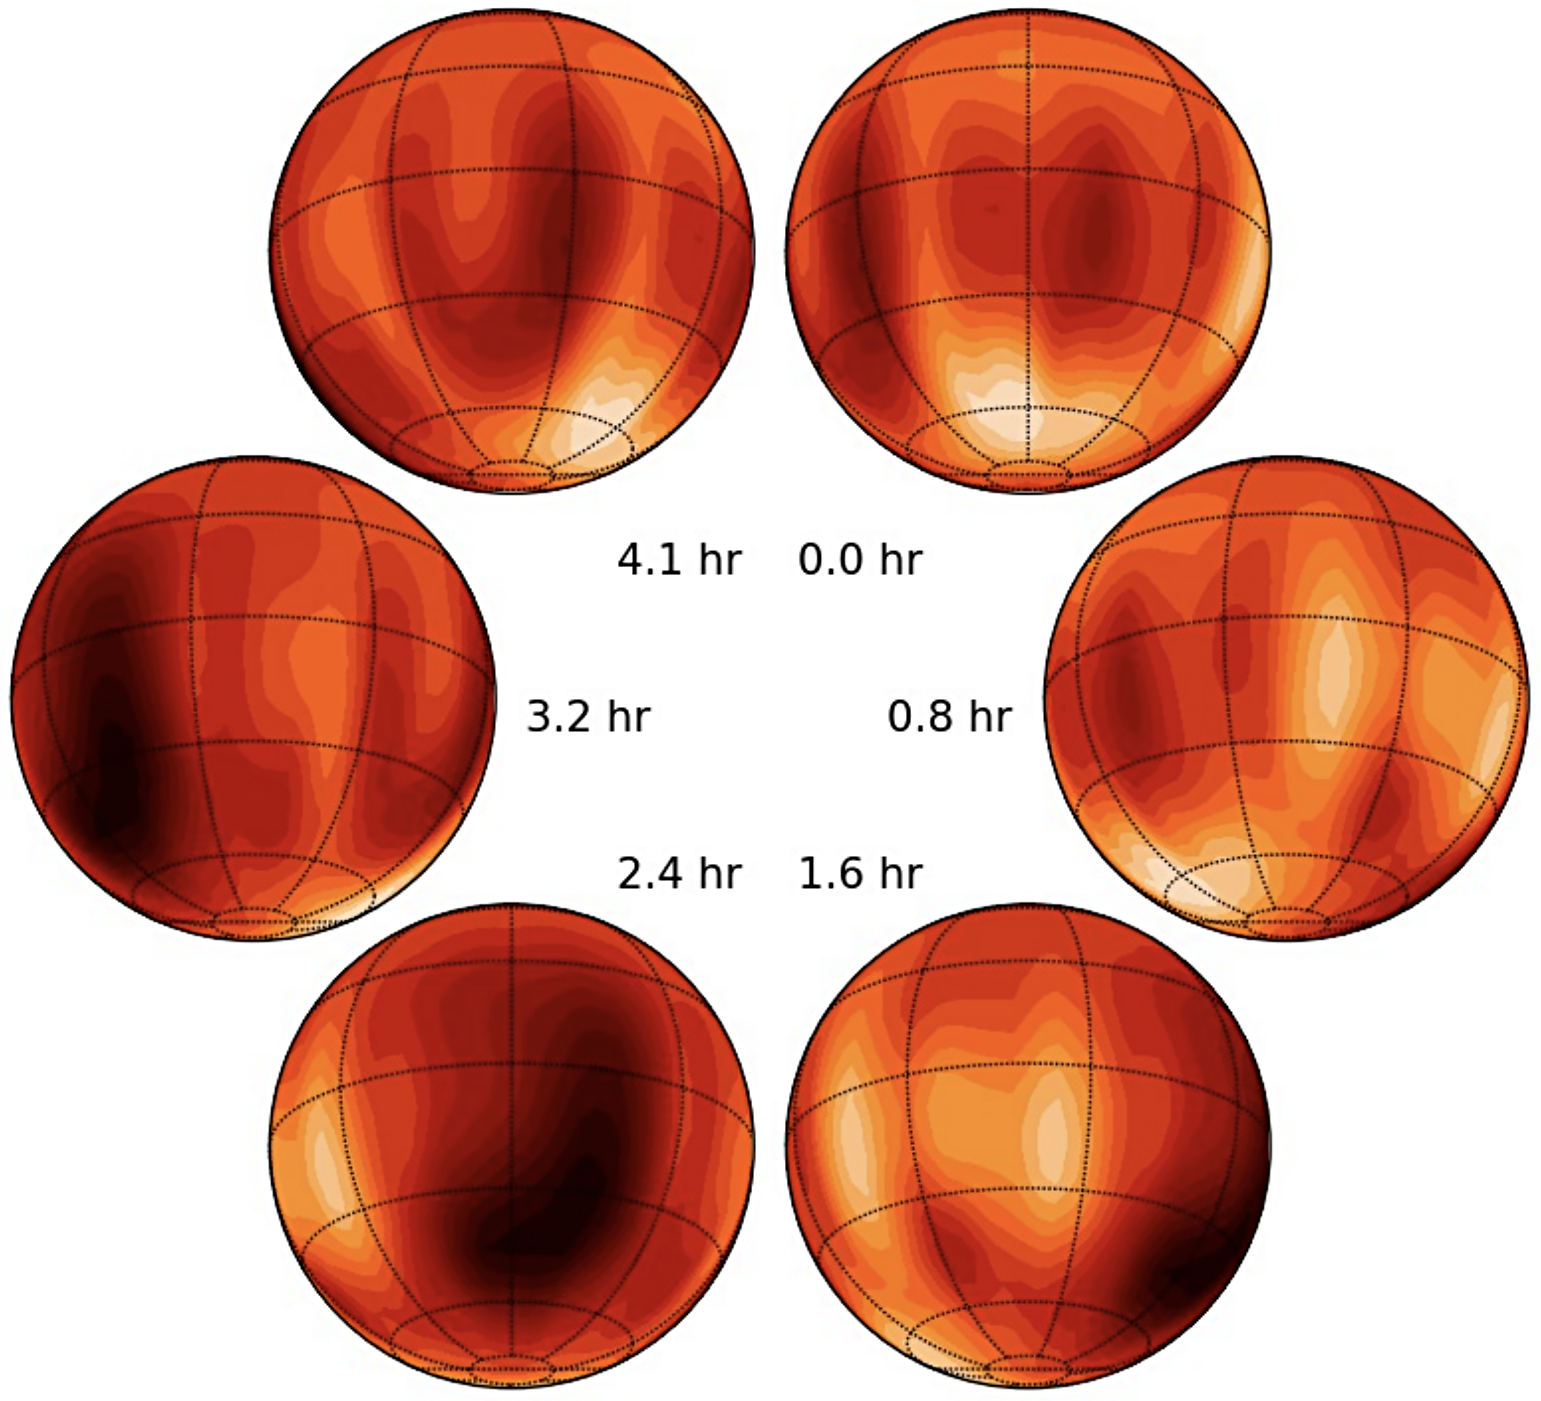
\includegraphics[width=0.462\linewidth]{static/luhman16b_crossfield.png} % 
        \caption{%
            Maximum \emph{a posteriori} surface maps of Luhman 16B inferred from the spectra in Figure~\ref{fig:luhman16b:data_model}. \emph{Left:} surface map inferred using the algorithm developed in this work. \emph{Right}: surface map inferred in \citet{Crossfield2014}, reproduced from Figure~2 in that paper.
            We infer the presence of a bright circumpolar spot, as well as the presence of a few dark features, most of which agree with the map presented in the original work.
        }
        \label{fig:luhman16b:maps}
    \end{centering}
\end{figure}

Our results are shown in Figures~\ref{fig:luhman16b:data_model}, \ref{fig:luhman16b:template_spectra}, and \ref{fig:luhman16b:maps}.
In Figure~\ref{fig:luhman16b:data_model}, our maximum \emph{a posteriori} (MAP) model for each of the 14 spectra is shown as the orange line; it agrees with the data to within the measurement uncertainties.
In Figure~\ref{fig:luhman16b:template_spectra} we show our MAP \emph{template} (rest frame) spectrum as the orange curve.
Since we used the \citet{Crossfield2014} template as a prior (blue curve), our solution is very similar to the input spectrum.
Nevertheless, we infer slightly different line depths for several of the lines at the level of a few percent; we also infer slightly different continuum levels in certain portions of the spectrum.
Note, importantly, since we only performed an optimization (rather than full posterior inference), we cannot quantify the actual significance of these differences.

The right panel of Figure~\ref{fig:luhman16b:maps} shows our principal result: the inferred solution for the surface brightness map of Luhman 16B; compare to the right panel, showing the solution inferred by \citet{Crossfield2014}.
Broadly speaking, the two surface maps agree rather well: we infer the same circumpolar bright spot, of about the same size and at roughly the same phase, although the exact latitude is different.
We also infer a similar dark feature on the ``back'' side of the object (visible near the sub-observer point at $t = 2.4$ hours).
Bright equatorial regions also broadly match between both solutions.
There are some important differences, such as the behavior of the $t = 2.4$ hour dark region beyond $60^\circ$ of the visible pole.
In general, we find that different choices for our priors---in particular the regularization on the pixels and the template spectrum, the prior on the limb darkening coefficient, and the value of the inclination of the star---result in maps that differ somewhat.
We do, however, agree with \citet{Crossfield2014} in that the polar bright spot is the most robust of the inferred features, followed by the bottom portion of the dark spot seen at $t = 2.4$ hours.
Once again, since this is simply an \emph{optimization}, we are unable to place reliable uncertainties on our solutions.
These require a sampling scheme like MCMC (\S\ref{sec:discussion:priors}).


\section{Discussion}
\label{sec:discussion}
%

\subsection{Luhman 16B}
\label{sec:discussion:luhman}

In \S\ref{sec:luhman16b} we validated our novel approach by reproducing the results of \citet{Crossfield2014}. 
Despite the fact that we obtained a qualitatively similar surface map for Luhman 16B (Figure~\ref{fig:luhman16b:maps}), there are several aspects to our approach that could be improved in future work. 
%
First, we did not vary the inclination, but instead kept it fixed at the fiducial value $i = 70^\circ$ used in \citet{Crossfield2014}. 
The authors of that study argued that the SNR of the dataset was too low to constrain the inclination, and that their surface maps did not qualitatively change by varying the inclination between $60^\circ$ and $90^\circ$, the range consistent with the joint knowledge of the rotation period and $v\sin i$. 
We find a similar result, but we note that the likelihood of the solution improves marginally when we allow the inclination to vary.
A posterior inference scheme may thus be able to place stronger constraints on the value of $i$.
%
Second, neither our study nor that of \citet{Crossfield2014} accounted for the finite exposure time of the observations; given that each of the 14 spectra were collected over 20 minutes, the object rotates through $\frac{20\,\mathrm{min}}{4.9\,\mathrm{hr}}\times 360^\circ \approx 24^\circ$ during each exposure.
Nevertheless, this is comparable to the limiting resolution of our $l_\mathrm{max} = 10$ spherical harmonic expansion (equal to about $180^\circ / l_\mathrm{max} = 18^\circ$), so it is unlikely to substantially change our results.
%
Third, as in \citet{Crossfield2014}, we accounted for instrumental broadening in the template spectrum; in other words, the spectrum shown in Figure~\ref{fig:luhman16b:template_spectra}, the input into our Doppler imaging code, includes broadening due to the finite spectral resolution of CRIRES.
A better approach is to compute the Doppler-broadened spectrum based on the true rest frame spectrum and \emph{then} apply instrumental broadening (i.e., the order in which events take place in reality).
%
Finally, and most importantly, our results (like those of \citet{Crossfield2014}) are just a point estimate.
While the main features inferred in the map---the polar bright spot and the dark spot on the back side of the object---appear to be robust to changes in our priors, we are unable to quantify our confidence in the map solution.
%
Doing so is straightforward with the \starry implementation of our algorithm, but we defer it to future work.

\subsection{Regularization, priors, and posteriors}
\label{sec:discussion:priors}
%
\subsubsection{Gaussian priors}
\label{sec:discussion:priors:gaussian}
%
In \S\ref{sec:spotstar} we took advantage of the bilinear nature of the problem to compute the uncertainty (\S\ref{sec:spot_y1}) and lower bounds on the uncertainty (\S\ref{sec:spot_y1b} and \S\ref{sec:spot_y1bs}) of the surface map solution. 
In particular, we found that the posterior uncertainty on the map ranges from about one percent at the north (visible) pole of the star to upwards of 10 percent at the south (hidden) pole (see Figures~\ref{fig:spot_infer_y}--\ref{fig:spot_infer_ybs}).
It is important to keep in mind that these values are entirely dependent on our choice of prior (namely, a zero-mean Gaussian prior on the spherical harmonic coefficients with constant variance equal to $10^{-4}$).
In particular, the value of the posterior uncertainty close to the south pole of the star---which is never in view, and whose true intensity cannot be constrained from the data---is determined exclusively from the prior variance we chose above (via Equation~\ref{eq:spotstar:uncert}).
Its value is therefore as arbitrary as our choice of prior.%
\footnote{While the exact \emph{value} of the posterior variance scales with the prior variance, the \emph{ratio} between the uncertainty in the north and the south does not. 
The gradient seen in the uncertainty maps of Figures~\ref{fig:spot_infer_y}--\ref{fig:spot_infer_ybs} \emph{is} therefore meaningful, as it directly encodes the spatial distribution of the information content of the data.}
In \S\ref{sec:spotstar} we chose a variance of $10^{-4}$ because we had access to the true maps and found, via trial and error, that this value yielded a good balance between underfitting and overfitting the synthetic data. In a realistic application, however, we could not do this, so we must naturally wonder: how should we go about choosing the prior variance in a principled way?

There are (at least) two general approaches. 
The first, and most Bayesian, is to choose priors that truly encode our prior knowledge of the system. 
Absent prior observations of the system, these priors usually come from physics, such as our knowledge of the typical stellar photospheric temperatures or our understanding of the kinds of inhomogeneities we would expect on their surfaces (dark spots on stars, or patchy clouds on brown dwarfs). 
The most straightforward way to encode this information in our priors is to recognize that the prior variance on a spherical harmonic vector is closely related to a prior on its angular power spectrum \citep[see, e.g.,][]{Baldi2006,Wandelt2012}.
In particular, our choice for prior covariance in \S\ref{sec:spotstar}, namely $\boldsymbol{\Lambda}_\bvec{y} = 10^{-4}\bvec{I}$, implies an isotropic, flat angular power spectrum prior on our surface maps with power equal to $10^{-4}$ in each spherical harmonic degree.
Increasing this value will in general lead to solutions with more structure on all scales; decreasing it will favor more homogeneous maps.
This may be an acceptable prior if truly nothing is known about the typical angular scale of features on the surface, but this is seldom the case.
Both observations of the Sun and magnetohydrodynamic simulations of stellar magnetic fields give us prior constraints on the typical scales of starspots \xxx{(cite me)}, and climate models of brown dwarfs tell us about typical sizes of clouds and other atmospheric features \citep[e.g.,][]{Tan2019,Tan2020,Tan2021a,Tan2021b}.
These can be encoded into our Gaussian prior by choosing a prior variance that scales with spherical harmonic degree:
%
\begin{align}
    \boldsymbol{\Lambda}_\bvec{y} = 
    \begin{pmatrix}
        \sigma_0^2 & & & & & & & & & \\[-0.35em]
        & \sigma_1^2 & & & & & & & & \\[-0.35em]
        & & \sigma_1^2 & & & & & & & \\[-0.35em]
        & & & \sigma_1^2 & & & & & & \\[-0.35em]
        & & & & \sigma_2^2 & & & & & \\[-0.35em]
        & & & & & \sigma_2^2 & & & & \\[-0.35em]
        & & & & & & \sigma_2^2 & & & \\[-0.35em]
        & & & & & & & \sigma_2^2 & & \\[-0.35em]
        & & & & & & & & \sigma_2^2 & \\[-0.35em]
        & & & & & & & & & \ddots
    \end{pmatrix}
    \quad,
\end{align}
%
where the variance at each degree is parametrized as, e.g.,
%
\begin{align}
    \sigma_l^2(\alpha, \lambda, \tau) = \alpha^2 \exp\left(-\frac{(l - \lambda)^2}{2\tau^2}\right)
    \quad,
\end{align}
%
where $\lambda$ is the typical spherical harmonic degree of features, $\alpha^2$ is the prior variance at that degree, and $\tau$ controls the uncertainty in $\lambda$.
These hyperparameters can be either imposed or even \emph{learned} from the data; see below.

Sometimes, however, we may have even more information to encode in our priors, such as the typical \emph{latitude} of the features. This might be the case for Solar-like or low mass stars, which have specific active latitudes at which spots form. An isotropic prior of the form discussed above cannot encode this, but a dense covariance matrix (with structure in the off-diagonal elements) \emph{can}.


\xxx{Can use cross-validation to choose best regularization strength.
In general, a positivity prior on the pixels is preferred.}


\xxx{Discuss the case where the inclination/period/velocity is unknown, such as the case with Luhman 16B.
The problem is not linear in these variables, so we need MCMC. 
But our model is differentiable, so we can easily use HMC. 
Discuss.}

\subsection{Limitations and future work}
\label{sec:discussion:caveats}

We are not addressing differential rotation and convective blueshift.
These make the integral in Equation~(\ref{eq:deconv:kT}) very difficult to solve. 
We will tackle this in the next paper.
\xxx{...}

The instrumental profile is another Toeplitz matrix that can be dotted into Equation~(\ref{eq:linear:f}).
\xxx{...}

We are always integrating over the entire disk of the star.
Can integrate over the unocculted disk during an occultation (should actually be pretty trivial) so this can be used for Doppler tomography once I have some time to work it out!
\xxx{...}

Telluric lines could be learned from the data as in \citet{Bedell2019}.
\xxx{...}

\section{Implementation in \starry}
\label{sec:starry}

We implement the algorithm presented here in the \starry package \citep{Luger2019,Luger2021c}, an open-source \texttt{Python} library for stellar and planetary light curve analysis. 
All of the figures in this paper were generated via the Doppler imaging API in \starry. 
The scripts used to generate them are available on GitHub\footnote{\url{https://github.com/rodluger/paparazzi}} and can be directly accessed via the GitHub icons next to each figure caption.
These are well-commented and can be used as a starting point for other Doppler imaging projects.

The algorithm is implemented using \texttt{theano} \citep{Bergstra2010}, a just-in-time compiling framework for \texttt{Python} with powerful autodifferentiation and optimization capabilities.
As such, the algorithm is fully differentiable and thus easy to use within gradient-based optimization and/or inference schemes such as Hamiltonian Monte Carlo.
The analysis presented in Figures~\ref{fig:spot_infer_ybs} and \ref{fig:luhman16b:data_model}---\ref{fig:luhman16b:maps} harnesses this capability within the \texttt{pymc3} modeling framework; refer to the corresponding scripts for details.

The implementation of the algorithm in \starry is highly optimized.
Even though we derived the model for the flux as a purely linear operation on the spectral/spatial expansion of the stellar surface (Equation~\ref{eq:deconv:F}), it is more  efficient in practice to compute it as a convolution using the highly optimized \texttt{conv2d} operations in \texttt{theano}.
Typical runtimes and scalings for the \starry algorithm are shown in Figure~\ref{fig:runtime}, where we plot the evaluation of the full forward model for all spectra in a dataset as a function of several parameters.
%
\begin{figure}[t!]
    \begin{centering}
        \includegraphics[width=\linewidth]{figures/runtime.pdf}
        \caption{%
            Model evaluation time as a function of various parameters, for spherical harmonic degree $l_\mathrm{max} = 10$, $M = 10$ spectral epochs, $K = 200$ wavelength bins, and $v\sin i = 50$ km/s.
            Thin lines correspond to individual trials; the thick lines show the median evaluation time.
            Timing tests were performed on a 2-core Linux virtual GitHub Actions machine.
        }
        \label{fig:runtime}
    \end{centering}
\end{figure}
%
Equation~(\ref{eq:deconv:F}) requires first the rotation of the $(\lmax + 1)^2$ $\kT$ kernels (each of length $W$) to the correct stellar rotational phase, an operation that scales approximately as $W \lmax^3$, followed by $(\lmax + 1)^2$ linear convolutions of the rotated $\kT$ kernels with the spectral components (each of length $K$), which scales approximately as $W K \lmax^2$. 
Since typically $K \gg \lmax$, the latter computation dominates and the entire evaluation of the model for $M$ spectral epochs takes $\mathcal{O}(M W K \lmax^2)$ operations. 
This is consistent with the relationships shown in Figure~\ref{fig:runtime}: the runtime is linearly proportional to the number of spectral epochs $M$, the number of wavelength bins $K$, and the width of the convolution kernel $W \propto v\sin i$; and it scales quadratically with the degree of the spherical harmonic expansion $l_\mathrm{max}$.
In general, evalution of the model for a typical dataset takes on the order of 10 or a few tens of milliseconds.



\section{Conclusions}
\label{sec:conclusions}
%


\xxx{%
    \begin{enumerate}
        \item Advantages of data-driven modeling
        \item Interpretable priors
        \item Works on blended lines
        \item Uses the whole spectrum
        \item Yields uncertainties!
        \item Probably works on slow rotators
        \item Differentiable!
        \item Fast!
        \item Use in MCMC to marginalize over inclination and stuff
        \item Advertise showyourwork for open source papers!
        \item \citet{Crossfield2014b} and \citet{Snellen2014}: people talk seriously about making Doppler Imaging maps of directly-imaged planets like beta Pic b with the ELTs.  Those will be tough measurements but could be the first real, global​ maps of any planet beyond the solar system (sorry, but eclipse-mapping just doesn't quite cut it so far...).  So we need the best possible algorithms to maximize what we get our of the data.
        \item \citep{Tan2019,Tan2020,Tan2021a,Tan2021b}: Xianyu is the main person running simulations of brown dwarf global weather patterns, and the techniques outlined in your paper will offer the best way to test those models.
    \end{enumerate}
}


%
%
%
%
\clearpage
\appendix
%
%
%
%

\section{Solving the $\kT$ integral}
\label{app:kT}
%
In this section we will show how to compute the integral in Equation~(\ref{eq:kT:kT}), yielding the terms of the convolution kernel $\kT$. 
It is convenient to first change basis from spherical harmonics to polynomials on the sphere:
%
\begin{align}
    \label{eq:appendix:kT}
    \kT(\lnlam)
     & =
    \int\limits_{-\sqrt{1 - x^2}}^
    {\sqrt{1 - x^2}}
    \pbasis
    \Big(x, y\Big)
    \mathrm{d}y
    \,
    \AOne
    \nonumber \\[0.5em]
     & \equiv
    \rhoT(\lnlam)
    \,
    \AOne
    \quad,
\end{align}
%
where $\AOne$ is the change of basis matrix from spherical harmonics to polynomials \citep[Equation B11 in][]{Luger2019} and
%
\begin{align}
    \pbasis(\x) \equiv
    \Big(
    1 \quad\quad\quad\quad\quad\quad x \quad\quad\quad\quad\quad\quad z \quad\quad\quad\quad\quad\quad y \quad\quad\quad\quad\quad\quad x^2 \quad\quad\quad\quad\quad\quad xz \quad\quad\quad\quad\quad\quad xy \quad\quad\quad\quad\quad\quad yz \quad\quad\quad\quad\quad\quad y^2 \quad\quad\quad\quad\quad\quad
    ...
    \Big)^\top
    \quad,
\end{align}
%
is the polynomial basis \citep[Equation 7][]{Luger2019}.
The $n^\mathrm{th}$ term of the polynomial basis is a polynomial in $x$, $y$, and $z = \sqrt{1 - x^2 - y^2}$:
%
\begin{align}
    \pbasisn
    &=
    x^i y^j z^k
\end{align}
%
where $i, j, k$ are integers given by
%
\begin{align}
    \label{eq:kT:lm}
    i &= \floor*{\Lambda - \Delta}
    \nonumber \\[0.5em]
    j &= \floor*{\Delta}
    \nonumber \\[0.5em]
    k &= \ceil*{\Delta} - \floor*{\Delta}
\end{align}
%
with
%
\begin{align}
    \Lambda &= \floor*{\sqrt{n}}
    \nonumber \\[0.5em]
    \Delta &= \frac{n - \Lambda^2}{2}
    \quad .
\end{align}
%
We may now explicitly write down the $n^\mathrm{th}$ term of the vector $\rhoT(\lnlam)$ in Equation~(\ref{eq:appendix:kT}),
%
\begin{align}
    \label{eq:kT:sTexpression}
    \rho_n(\lnlam)
     & =
    \rho_{i,\,j,\,k}(\lnlam)
    =
    x^i
    \int\limits_{-\sqrt{1 - x^2}}^
    {\sqrt{1 - x^2}}
    y^j
    \left(1 - x^2 - y^2\right)^{\frac{k}{2}} \,
    \mathrm{d}y
    \quad .
\end{align}
%
When $i = k = 0$, the integral is easy to evaluate:
%
\begin{align}
    \rho_{i,\,j,\,0}(\lnlam_0)
     & =
    \begin{cases}
        2 \left( 1 - x^2 \right)^\frac{j + 1}{2}
        \quad\quad\quad\quad\quad\quad\quad\quad\quad\quad\quad\quad
          & j \, \mathrm{even}        \\
        0 & j \, \mathrm{odd} \quad .
    \end{cases}
\end{align}
%
The general term may be computed from the recurrence relation
%
\begin{align}
    \rho_{0,\,j,\,0}(\lnlam_0) = \frac{j - 1}{j + 1} \big(1 - x^2\big) \rho_{0,\,j-2,\,0}
\end{align}
%
provided
%
\begin{align}
    \rho_{0,\,0,\,0} & = 2 \sqrt{1-x^2} \nonumber \\
    \rho_{0,\,1,\,0} & = 0 \quad.
\end{align}
%
When $i = 0$ and $k = 1$, we may substitute $y = \sin\psi\sqrt{1 - x^2}$ in the integrand to obtain
%
\begin{align}
    \rho_{0,\,j,\,1}(\lnlam_0)
     & =
    (1 - x^2)^{\frac{j + 2}{2}}
    \int\limits_{-\frac{\pi}{2}}^{\frac{\pi}{2}}
    \sin^j\psi
    \cos^2\psi \,
    \mathrm{d}\psi
    \quad.
\end{align}
%
We may solve this integral using the recurrence relation
%
\begin{align}
    \int
    \sin^j\psi
    \cos^m\psi \,
    \mathrm{d}\psi
     & =
    -\frac{\sin^{j-1}\psi \cos^{m+1}\psi}{j + m}
    +
    \frac{j - 1}{j + m}\int\sin^{j-2}\psi \cos^m\psi \mathrm{d}\psi
    \quad ,
\end{align}
%
which, in our case, simplifies to
%
\begin{align}
    \int\limits_{-\frac{\pi}{2}}^{\frac{\pi}{2}}
    \sin^j\psi
    \cos^2\psi \,
    \mathrm{d}\psi
     & =
    \frac{j - 1}{j + 2}\int\limits_{-\frac{\pi}{2}}^
    {\frac{\pi}{2}}\sin^{j-2}\psi \cos^2\psi \mathrm{d}\psi
    \quad.
\end{align}
%
We thus arrive at the recurrence relation
%
\begin{align}
    \rho_{0,\,j,\,1} & = \frac{j - 1}{j + 2} \big(1 - x^2\big) \rho_{0,\,j-2,\,1}
\end{align}
%
with initial conditions
%
\begin{align}
    \rho_{0,\,0,\,1} & = \frac{\pi}{2} \big(1-x^2\big) \nonumber \\
    \rho_{0,\,1,\,1} & = 0 \quad.
\end{align}
%
Given these expressions, recursing upward in $i$ is easy:
%
\begin{align}
    \rho_{i,\,j,\,k} & = x \, \rho_{i-1,\,j,\,k} \quad.
\end{align}
%
This completes our derivation. 
To summarize, given the boundary conditions
%
\begin{align}
    \rho_{0,\,0,\,0} & = 2 \sqrt{1-x^2} \nonumber                \\
    \rho_{0,\,0,\,1} & = \frac{\pi}{2} \big(1-x^2\big) \nonumber \\
    \rho_{0,\,1,\,k} & = 0 \quad ,
\end{align}
%
we may compute any term in $\rhoT$ via the expressions
%
\begin{align}
    \label{eq:kT:sTrecurrence}
    \rho_{0,\,j,\,k} & = \frac{j - 1}{j + 1 + k} \big(1 - x^2\big) \rho_{0,\,j-2,\,k} \nonumber \\
    \rho_{i,\,j,\,k} & = x \, \rho_{i-1,\,j,\,k} \quad.
\end{align}
%
The terms of the convolution kernel $\kT$ are then obtained by dotting this vector into the change of basis matrix $\AOne$, as discussed above.

% Table
\clearpage
\begin{center}
    \begin{longtable}{cll}
        \caption{Common notation used in this paper}
        \label{tab:notation}                                                                                                                                            \\
        %
        \toprule
        \multicolumn{1}{c}{\textbf{Symbol}}                 &
        \multicolumn{1}{c}{\textbf{Description}}            &
        \multicolumn{1}{c}{\textbf{Reference}}                                                                                                                          \\
        \midrule
        \endfirsthead
        %
        \multicolumn{3}{c}%
        {{\bfseries \tablename\ \thetable{}}. (continued from previous page)}                                                                                           \\[0.5em]
        \toprule
        \multicolumn{1}{c}{\textbf{Symbol}}                 &
        \multicolumn{1}{c}{\textbf{Definition}}             &
        \multicolumn{1}{c}{\textbf{Reference}}                                                                                                                          \\
        \midrule
        \endhead
        \bottomrule
        %
        \endfoot
        %
        \endlastfoot
        %
        \midrule
        \multicolumn{3}{c}{\emph{Variables}}                                                                                                                            \\
        \midrule
        %
        $a_{lm}$                                            & spectral spherical harmonic coefficient                      & Equation~(\ref{eq:deconv:Ixi0})            \\
        $\almt$                                              & vector of spectral spherical harmonic coefficients          & Equation~(\ref{eq:deconv:almt})             \\
        $\bvec{A}$                                          & matrix form of $\bvec{a}$                                    & Equation~(\ref{eq:inverse:alm})          \\
        $\bvec{B}$                                          & baseline design matrix                                       & \S\ref{sec:norm}                 \\
        $c$                                                 & speed of light                                               & Equation~(\ref{eq:kT:beta})                \\
        $\Curve$                                            & curve of constant radial velocity                            & Equation~(\ref{eq:deconv:kT})              \\
        $\D$                                                & logarithmic Doppler shift                                    & Equation~(\ref{eq:the_problem:D})          \\
        $\Doppler$                                          & Doppler design matrix                                        & Equation~(\ref{eq:linear:f})               \\
        $\bvec{f}$                                          & vector of observed flux values                               & Equation~(\ref{eq:linear:f})               \\
        $F$                                                 & flux                                                         & Equation~(\ref{eq:the_problem:F})          \\
        $i$                                                 & inclination                                                  & Equation~(\ref{eq:kT:beta})                \\
        $I$                                                 & specific intensity                                           & Equation~(\ref{eq:the_problem:Ixi})        \\
        $\bvec{I}$                                          & identity matrix                                              &                                            \\
        $l$                                                 & spherical harmonic degree                                    &                                            \\
        $\bvec{L}$                                          & limb darkening operator                                      & Equation~(\ref{eq:ld:L})                   \\
        $m$                                                 & spherical harmonic order                                     &                                            \\
        $\bvec{P}$                                          & Change of basis matrix from $Y_{lm}$ to pixels               & Equation~(\ref{eq:spotstar:uncert})        \\
        $\bvec{R}$                                          & Wigner rotation matrix                                       & Equation~(\ref{eq:deconv:R})               \\
        $\bvec{s}$                                          & vector representation of the spectrum                        & Equation~(\ref{eq:inverse:alm})          \\
        $\bvec{S}$                                          & block matrix representation of $\bvec{s}$                    & Equation~(\ref{eq:inverse:S})              \\
        $\boldsymbol{\mathbb{S}}$                           & matrix of $J$ spectral components                            & Equation~(\ref{eq:eigen:alm})            \\
        $\Surf$                                             & projected visible area of the star                           & Equation~(\ref{eq:the_problem:F})          \\
        $t$                                                 & time                                                         & \S\ref{sec:the_problem}                    \\
        $T$                                                 & artificial temperature in bilinear solver                    & \S\ref{sec:spotstar}                       \\
        $T_0$                                               & initial artificial temperature setting                       & \S\ref{sec:spotstar}                       \\
        $\Delta\log T$                                      & artificial temperature step size                             & \S\ref{sec:spotstar}                       \\
        $u$                                                 & limb darkening coefficient                                   & \S\ref{sec:ld}                             \\
        $\x$                                                & Cartesian position on the sky                                & \S\ref{sec:the_problem}                    \\
        $y_{lm}$                                            & spherical harmonic coefficient                               & \S\ref{sec:inverse}                        \\
        $\bvec{y}$                                          & vector of spherical harmonic coefficients                    & Equation~(\ref{eq:inverse:alm})          \\
        $Y_{lm}$                                            & spherical harmonic                                           & Equation~(\ref{eq:deconv:Ixi0})            \\
        $\bvec{Y}$                                          & block matrix representation of $\bvec{y}$                    & Equation~(\ref{eq:inverse:Y})              \\
        $\boldsymbol{\mathbb{Y}}$                           & matrix of $J$ spherical harmonic components                  & Equation~(\ref{eq:eigen:alm})            \\
        %
        \pagebreak
        \midrule
        \multicolumn{3}{c}{\emph{Variables (Greek)}}                                                                                                                    \\
        \midrule
        %
        $\beta$                                             & relativistic parameter                                       & Equation~(\ref{eq:the_problem:D})          \\
        $\delta$                                            & Dirac delta function                                         & Equation~(\ref{eq:deconv:convolution})     \\
        $\kT$                                               & convolution kernel basis vector                              & Equation~(\ref{eq:deconv:kT})              \\
        $\lambda$                                           & wavelength                                                   & \S\ref{sec:the_problem}                    \\
        $\lambda_\mathrm{r}$                                & reference wavelength                                         & \S\ref{sec:the_problem}                    \\
        $\lnlam$                                            & $\ln\frac{\lambda}{\lambda_\mathrm{r}}$ (observer frame)     & \S\ref{sec:the_problem}                    \\
        $\lnlam_0$                                          & $\ln\frac{\lambda}{\lambda_\mathrm{r}}$ (rest frame)         & \S\ref{sec:the_problem}                    \\
        $\boldsymbol{\Lambda}$                              & prior covariance matrix                                      &                                            \\
        $\boldsymbol{\mu}$                                  & prior mean vector                                            &                                            \\
        $\ylmbasis$                                         & spherical harmonic basis vector                              & Equation~(\ref{eq:deconv:ylmbasis})        \\
        $\boldsymbol{\Sigma}$                               & covariance matrix                                            &                                            \\
        $\omega$                                            & angular velocity                                             & Equation~(\ref{eq:kT:beta})                \\
        %
        \midrule
        \multicolumn{3}{c}{\emph{Dimensions}}                                                                                                                           \\
        \midrule
        %
        $J$                                                 & \# of spectral components                                    & \S\ref{sec:eigen}                          \\
        $K$                                                 & \# of wavelength bins in the broadened spectrum              & \S\ref{sec:linear}                         \\
        $K'$                                                & \# of wavelength bins in the latent spectrum                 & \S\ref{sec:linear}                         \\
        $K_\mathrm{obs}$                                    & \# of wavelength bins in the observed spectrum               & \S\ref{sec:spotstar}                       \\
        $M$                                                 & \# of epochs observed                                        & \S\ref{sec:linear}                         \\
        $N$                                                 & \# of spherical harmonic coefficients                        & \S\ref{sec:linear}                         \\
        $N'$                                                & \# of spherical harmonic coefficients after limb darkening   & \S\ref{sec:ld}                             \\
        $W$                                                 & \# of wavelength bins in the convolution kernel              & \S\ref{sec:linear}                         \\
        %
        \midrule
        \multicolumn{3}{c}{\emph{Operators \& Other symbols}}                                                                                                           \\
        \midrule
        %
        $\mathrm{diag}$                                     & diagonal matricization                                       & Equation~(\ref{eq:ld:Dmwav})               \\
        $\mathrm{vec}$                                      & vectorization                                                & Equation~(\ref{eq:inverse:alm})          \\
        $*$                                                 & convolution                                                  & Equation~(\ref{eq:deconv:convolution_def}) \\
        $\circ$                                             & element-wise product                                         & \S\ref{sec:norm}           \\
        $\otimes$                                           & Kronecker product                                            & Equation~(\ref{eq:linear:Dm})              \\
        $\ceil*{\,}$                                        & ceiling                                                      & Equation~(\ref{eq:kT:lm})                  \\
        $\floor*{\,}$                                       & floor                                                        & Equation~(\ref{eq:kT:lm})                  \\
        $\bvec{0}$                                          & the zero vector, $(0 \quadquad 0 \quadquad \cdots \quadquad 0)^\top$ &                                                                                                           \\
        $\bvec{1}$                                          & the one vector, $(1 \quadquad 1 \quadquad \cdots \quadquad 1)^\top$ &                                                                                                           \\
    \end{longtable}
\end{center}

% Bibliography
\clearpage
\bibliography{bib}

\end{document}